\subsection{Четвёртое БДЗ}


\setcounter{iii}{15}

\i \textbf{(4).}
\begin{gather*}
    \frac{1}{e^{(x^2+2x)(x+3)^2}};
    \intertext{Заметим, что наша функция имеет вид <<константа делить на непрерывную функцию>>, а значит может быть разрывна только в тех точках, в которых знаменатель равен или стремится к нулю:}
    \begin{cases}
        e^{(x^2+2x)(x+3)^2} = 0, & \text{очевидно, не имеет решений,}\\
        \limit{x}{x_0} e^{(x^2+2x)(x+3)^2} = 0, & \text{рассмотрим отдельно;}
    \end{cases}\\
    \limit{x}{x_0} e^{(x^2+2x)(x+3)^2} = 0 <=> \limit{x}{x_0} (x^2+2x)(x+3)^2 = -\infty;\\
    \limit{x}{x_0} (x^2+2x)(x+3)^2 = -\infty;
\end{gather*} 
не имеет решений в силу того, что рассматриваетмая функция является многочленом чётной степени, а значит ни в какой точке не стемится к $-\infty$.
Таким образом, данная функция является непрерывной на всей числовой оси.\\
Эскиз графика:\\
\pgfplotsset{width=20cm, compat=1.15}
\usetikzlibrary{arrows}
\pagestyle{empty}
 
%<<<<<<<WARNING>>>>>>>
% PGF/Tikz doesn't support the following mathematical functions:
% cosh, acosh, sinh, asinh, tanh, atanh,
% x^r with r not integer

% Plotting will be done using GNUPLOT
% GNUPLOT must be installed and you must allow Latex to call external
% programs by adding the following option to your compiler
% shell-escape    OR    enable-write18 
% Example: pdflatex --shell-escape file.tex 

\definecolor{qqwuqq}{rgb}{0.75,0,0}
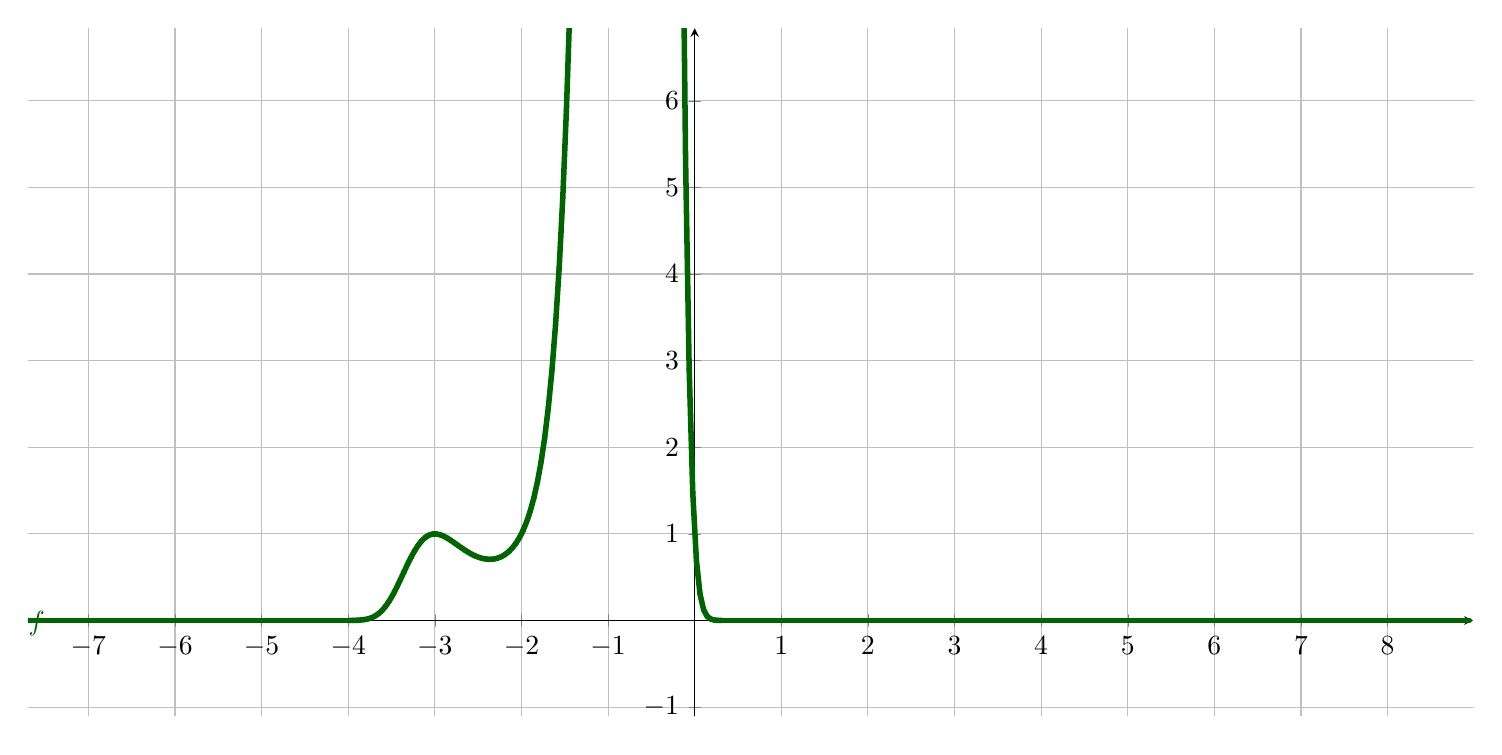
\begin{tikzpicture}[line cap=round,line join=round,>=triangle 45,x=1.1cm,y=1.1cm]
\begin{axis}[
x=1.1cm,y=1.1cm,
axis lines=middle,
ymajorgrids=true,
xmajorgrids=true,
xmin=-7.6943635820329135,
xmax=8.984547313382953,
ymin=-1.1,
ymax=6.837745000369829,
xtick={-7,-6,...,8},
ytick={-1,-0,...,6},]
\clip(-7.6943635820329135,-4.0928206256076445) rectangle (8.984547313382953,6.837745000369829);
\draw[line width=2pt,color=qqwuqq] (-7.6943635820329135,0) -- (-7.6943635820329135,0);
\draw[line width=2pt,color=qqwuqq] (-7.6943635820329135,0) -- (-7.652666304794374,0);
\draw[line width=2pt,color=qqwuqq] (-7.652666304794374,0) -- (-7.610969027555834,0);
\draw[line width=2pt,color=qqwuqq] (-7.610969027555834,0) -- (-7.569271750317294,0);
\draw[line width=2pt,color=qqwuqq] (-7.569271750317294,0) -- (-7.527574473078754,0);
\draw[line width=2pt,color=qqwuqq] (-7.527574473078754,0) -- (-7.485877195840215,0);
\draw[line width=2pt,color=qqwuqq] (-7.485877195840215,0) -- (-7.444179918601675,0);
\draw[line width=2pt,color=qqwuqq] (-7.444179918601675,0) -- (-7.402482641363135,0);
\draw[line width=2pt,color=qqwuqq] (-7.402482641363135,0) -- (-7.360785364124595,0);
\draw[line width=2pt,color=qqwuqq] (-7.360785364124595,0) -- (-7.3190880868860555,0);
\draw[line width=2pt,color=qqwuqq] (-7.3190880868860555,0) -- (-7.277390809647516,0);
\draw[line width=2pt,color=qqwuqq] (-7.277390809647516,0) -- (-7.235693532408976,0);
\draw[line width=2pt,color=qqwuqq] (-7.235693532408976,0) -- (-7.193996255170436,0);
\draw[line width=2pt,color=qqwuqq] (-7.193996255170436,0) -- (-7.152298977931896,0);
\draw[line width=2pt,color=qqwuqq] (-7.152298977931896,0) -- (-7.110601700693357,0);
\draw[line width=2pt,color=qqwuqq] (-7.110601700693357,0) -- (-7.068904423454817,0);
\draw[line width=2pt,color=qqwuqq] (-7.068904423454817,0) -- (-7.027207146216277,0);
\draw[line width=2pt,color=qqwuqq] (-7.027207146216277,0) -- (-6.985509868977737,0);
\draw[line width=2pt,color=qqwuqq] (-6.985509868977737,0) -- (-6.9438125917391975,0);
\draw[line width=2pt,color=qqwuqq] (-6.9438125917391975,0) -- (-6.902115314500658,0);
\draw[line width=2pt,color=qqwuqq] (-6.902115314500658,0) -- (-6.860418037262118,0);
\draw[line width=2pt,color=qqwuqq] (-6.860418037262118,0) -- (-6.818720760023578,0);
\draw[line width=2pt,color=qqwuqq] (-6.818720760023578,0) -- (-6.777023482785038,0);
\draw[line width=2pt,color=qqwuqq] (-6.777023482785038,0) -- (-6.735326205546499,0);
\draw[line width=2pt,color=qqwuqq] (-6.735326205546499,0) -- (-6.693628928307959,0);
\draw[line width=2pt,color=qqwuqq] (-6.693628928307959,0) -- (-6.651931651069419,0);
\draw[line width=2pt,color=qqwuqq] (-6.651931651069419,0) -- (-6.610234373830879,0);
\draw[line width=2pt,color=qqwuqq] (-6.610234373830879,0) -- (-6.5685370965923395,0);
\draw[line width=2pt,color=qqwuqq] (-6.5685370965923395,0) -- (-6.5268398193538,0);
\draw[line width=2pt,color=qqwuqq] (-6.5268398193538,0) -- (-6.48514254211526,0);
\draw[line width=2pt,color=qqwuqq] (-6.48514254211526,0) -- (-6.44344526487672,0);
\draw[line width=2pt,color=qqwuqq] (-6.44344526487672,0) -- (-6.40174798763818,0);
\draw[line width=2pt,color=qqwuqq] (-6.40174798763818,0) -- (-6.360050710399641,0);
\draw[line width=2pt,color=qqwuqq] (-6.360050710399641,0) -- (-6.318353433161101,0);
\draw[line width=2pt,color=qqwuqq] (-6.318353433161101,0) -- (-6.276656155922561,0);
\draw[line width=2pt,color=qqwuqq] (-6.276656155922561,0) -- (-6.234958878684021,0);
\draw[line width=2pt,color=qqwuqq] (-6.234958878684021,0) -- (-6.1932616014454815,0);
\draw[line width=2pt,color=qqwuqq] (-6.1932616014454815,0) -- (-6.151564324206942,0);
\draw[line width=2pt,color=qqwuqq] (-6.151564324206942,0) -- (-6.109867046968402,0);
\draw[line width=2pt,color=qqwuqq] (-6.109867046968402,0) -- (-6.068169769729862,0);
\draw[line width=2pt,color=qqwuqq] (-6.068169769729862,0) -- (-6.026472492491322,0);
\draw[line width=2pt,color=qqwuqq] (-6.026472492491322,0) -- (-5.984775215252783,0);
\draw[line width=2pt,color=qqwuqq] (-5.984775215252783,0) -- (-5.943077938014243,0);
\draw[line width=2pt,color=qqwuqq] (-5.943077938014243,0) -- (-5.901380660775703,0);
\draw[line width=2pt,color=qqwuqq] (-5.901380660775703,0) -- (-5.859683383537163,0);
\draw[line width=2pt,color=qqwuqq] (-5.859683383537163,0) -- (-5.817986106298624,0);
\draw[line width=2pt,color=qqwuqq] (-5.817986106298624,0) -- (-5.776288829060084,0);
\draw[line width=2pt,color=qqwuqq] (-5.776288829060084,0) -- (-5.734591551821544,0);
\draw[line width=2pt,color=qqwuqq] (-5.734591551821544,0) -- (-5.692894274583004,0);
\draw[line width=2pt,color=qqwuqq] (-5.692894274583004,0) -- (-5.6511969973444645,0);
\draw[line width=2pt,color=qqwuqq] (-5.6511969973444645,0) -- (-5.609499720105925,0);
\draw[line width=2pt,color=qqwuqq] (-5.609499720105925,0) -- (-5.567802442867385,0);
\draw[line width=2pt,color=qqwuqq] (-5.567802442867385,0) -- (-5.526105165628845,0);
\draw[line width=2pt,color=qqwuqq] (-5.526105165628845,0) -- (-5.484407888390305,0);
\draw[line width=2pt,color=qqwuqq] (-5.484407888390305,0) -- (-5.442710611151766,0);
\draw[line width=2pt,color=qqwuqq] (-5.442710611151766,0) -- (-5.401013333913226,0);
\draw[line width=2pt,color=qqwuqq] (-5.401013333913226,0) -- (-5.359316056674686,0);
\draw[line width=2pt,color=qqwuqq] (-5.359316056674686,0) -- (-5.317618779436146,0);
\draw[line width=2pt,color=qqwuqq] (-5.317618779436146,0) -- (-5.2759215021976065,0);
\draw[line width=2pt,color=qqwuqq] (-5.2759215021976065,0) -- (-5.234224224959067,0);
\draw[line width=2pt,color=qqwuqq] (-5.234224224959067,0) -- (-5.192526947720527,0);
\draw[line width=2pt,color=qqwuqq] (-5.192526947720527,0) -- (-5.150829670481987,0);
\draw[line width=2pt,color=qqwuqq] (-5.150829670481987,0) -- (-5.109132393243447,0);
\draw[line width=2pt,color=qqwuqq] (-5.109132393243447,0) -- (-5.067435116004908,0);
\draw[line width=2pt,color=qqwuqq] (-5.067435116004908,0) -- (-5.025737838766368,0);
\draw[line width=2pt,color=qqwuqq] (-5.025737838766368,0) -- (-4.984040561527828,0);
\draw[line width=2pt,color=qqwuqq] (-4.984040561527828,0) -- (-4.942343284289288,0);
\draw[line width=2pt,color=qqwuqq] (-4.942343284289288,0) -- (-4.9006460070507485,0);
\draw[line width=2pt,color=qqwuqq] (-4.9006460070507485,0) -- (-4.858948729812209,0);
\draw[line width=2pt,color=qqwuqq] (-4.858948729812209,0) -- (-4.817251452573669,0);
\draw[line width=2pt,color=qqwuqq] (-4.817251452573669,0) -- (-4.775554175335129,0);
\draw[line width=2pt,color=qqwuqq] (-4.775554175335129,0) -- (-4.733856898096589,0);
\draw[line width=2pt,color=qqwuqq] (-4.733856898096589,0) -- (-4.69215962085805,0);
\draw[line width=2pt,color=qqwuqq] (-4.69215962085805,0) -- (-4.65046234361951,0);
\draw[line width=2pt,color=qqwuqq] (-4.65046234361951,0) -- (-4.60876506638097,0);
\draw[line width=2pt,color=qqwuqq] (-4.60876506638097,0) -- (-4.56706778914243,0);
\draw[line width=2pt,color=qqwuqq] (-4.56706778914243,0) -- (-4.5253705119038905,0);
\draw[line width=2pt,color=qqwuqq] (-4.5253705119038905,0) -- (-4.483673234665351,0);
\draw[line width=2pt,color=qqwuqq] (-4.483673234665351,0) -- (-4.441975957426811,0);
\draw[line width=2pt,color=qqwuqq] (-4.441975957426811,0) -- (-4.400278680188271,0);
\draw[line width=2pt,color=qqwuqq] (-4.400278680188271,0) -- (-4.358581402949731,0);
\draw[line width=2pt,color=qqwuqq] (-4.358581402949731,0) -- (-4.316884125711192,0);
\draw[line width=2pt,color=qqwuqq] (-4.316884125711192,0) -- (-4.275186848472652,0);
\draw[line width=2pt,color=qqwuqq] (-4.275186848472652,0) -- (-4.233489571234112,0);
\draw[line width=2pt,color=qqwuqq] (-4.233489571234112,0) -- (-4.191792293995572,0);
\draw[line width=2pt,color=qqwuqq] (-4.191792293995572,0) -- (-4.1500950167570325,0);
\draw[line width=2pt,color=qqwuqq] (-4.1500950167570325,0) -- (-4.108397739518493,0);
\draw[line width=2pt,color=qqwuqq] (-4.108397739518493,0) -- (-4.066700462279953,0);
\draw[line width=2pt,color=qqwuqq] (-4.066700462279953,0) -- (-4.025003185041413,0);
\draw[line width=2pt,color=qqwuqq] (-4.025003185041413,0) -- (-3.9833059078028734,0);
\draw[line width=2pt,color=qqwuqq] (-3.9833059078028734,0) -- (-3.9416086305643336,0.0011301449471370023);
\draw[line width=2pt,color=qqwuqq] (-3.9416086305643336,0.0011301449471370023) -- (-3.899911353325794,0.0024775098519142424);
\draw[line width=2pt,color=qqwuqq] (-3.899911353325794,0.0024775098519142424) -- (-3.858214076087254,0.005089991256789512);
\draw[line width=2pt,color=qqwuqq] (-3.858214076087254,0.005089991256789512) -- (-3.8165167988487143,0.009832387664556345);
\draw[line width=2pt,color=qqwuqq] (-3.8165167988487143,0.009832387664556345) -- (-3.7748195216101745,0.01791552996233115);
\draw[line width=2pt,color=qqwuqq] (-3.7748195216101745,0.01791552996233115) -- (-3.7331222443716348,0.030887725259406924);
\draw[line width=2pt,color=qqwuqq] (-3.7331222443716348,0.030887725259406924) -- (-3.691424967133095,0.05054208726330549);
\draw[line width=2pt,color=qqwuqq] (-3.691424967133095,0.05054208726330549) -- (-3.649727689894555,0.0787272852307791);
\draw[line width=2pt,color=qqwuqq] (-3.649727689894555,0.0787272852307791) -- (-3.6080304126560154,0.1170751164699144);
\draw[line width=2pt,color=qqwuqq] (-3.6080304126560154,0.1170751164699144) -- (-3.5663331354174757,0.16668710271121212);
\draw[line width=2pt,color=qqwuqq] (-3.5663331354174757,0.16668710271121212) -- (-3.524635858178936,0.22784359388905115);
\draw[line width=2pt,color=qqwuqq] (-3.524635858178936,0.22784359388905115) -- (-3.482938580940396,0.29980364706241847);
\draw[line width=2pt,color=qqwuqq] (-3.482938580940396,0.29980364706241847) -- (-3.4412413037018563,0.380748847414324);
\draw[line width=2pt,color=qqwuqq] (-3.4412413037018563,0.380748847414324) -- (-3.3995440264633165,0.4678931664811681);
\draw[line width=2pt,color=qqwuqq] (-3.3995440264633165,0.4678931664811681) -- (-3.3578467492247768,0.5577435307391213);
\draw[line width=2pt,color=qqwuqq] (-3.3578467492247768,0.5577435307391213) -- (-3.316149471986237,0.6464633689579908);
\draw[line width=2pt,color=qqwuqq] (-3.316149471986237,0.6464633689579908) -- (-3.274452194747697,0.7302728233513119);
\draw[line width=2pt,color=qqwuqq] (-3.274452194747697,0.7302728233513119) -- (-3.2327549175091574,0.8058180374855974);
\draw[line width=2pt,color=qqwuqq] (-3.2327549175091574,0.8058180374855974) -- (-3.1910576402706177,0.8704558306762508);
\draw[line width=2pt,color=qqwuqq] (-3.1910576402706177,0.8704558306762508) -- (-3.149360363032078,0.9224231087145589);
\draw[line width=2pt,color=qqwuqq] (-3.149360363032078,0.9224231087145589) -- (-3.107663085793538,0.960885314348226);
\draw[line width=2pt,color=qqwuqq] (-3.107663085793538,0.960885314348226) -- (-3.0659658085549983,0.9858790523997902);
\draw[line width=2pt,color=qqwuqq] (-3.0659658085549983,0.9858790523997902) -- (-3.0242685313164586,0.9981772585686638);
\draw[line width=2pt,color=qqwuqq] (-3.0242685313164586,0.9981772585686638) -- (-2.982571254077919,0.9991101969915976);
\draw[line width=2pt,color=qqwuqq] (-2.982571254077919,0.9991101969915976) -- (-2.940873976839379,0.9903735442696046);
\draw[line width=2pt,color=qqwuqq] (-2.940873976839379,0.9903735442696046) -- (-2.8991766996008392,0.9738483007985589);
\draw[line width=2pt,color=qqwuqq] (-2.8991766996008392,0.9738483007985589) -- (-2.8574794223622995,0.9514488511683382);
\draw[line width=2pt,color=qqwuqq] (-2.8574794223622995,0.9514488511683382) -- (-2.8157821451237597,0.9250072608892377);
\draw[line width=2pt,color=qqwuqq] (-2.8157821451237597,0.9250072608892377) -- (-2.77408486788522,0.8961951618392116);
\draw[line width=2pt,color=qqwuqq] (-2.77408486788522,0.8961951618392116) -- (-2.73238759064668,0.8664799035775961);
\draw[line width=2pt,color=qqwuqq] (-2.73238759064668,0.8664799035775961) -- (-2.6906903134081404,0.8371090179314903);
\draw[line width=2pt,color=qqwuqq] (-2.6906903134081404,0.8371090179314903) -- (-2.6489930361696006,0.8091161035245183);
\draw[line width=2pt,color=qqwuqq] (-2.6489930361696006,0.8091161035245183) -- (-2.607295758931061,0.7833414924506594);
\draw[line width=2pt,color=qqwuqq] (-2.607295758931061,0.7833414924506594) -- (-2.565598481692521,0.7604620295683187);
\draw[line width=2pt,color=qqwuqq] (-2.565598481692521,0.7604620295683187) -- (-2.5239012044539813,0.7410255819562298);
\draw[line width=2pt,color=qqwuqq] (-2.5239012044539813,0.7410255819562298) -- (-2.4822039272154415,0.7254872257379226);
\draw[line width=2pt,color=qqwuqq] (-2.4822039272154415,0.7254872257379226) -- (-2.4405066499769017,0.7142452657149861);
\draw[line width=2pt,color=qqwuqq] (-2.4405066499769017,0.7142452657149861) -- (-2.398809372738362,0.7076762557636541);
\draw[line width=2pt,color=qqwuqq] (-2.398809372738362,0.7076762557636541) -- (-2.357112095499822,0.7061689931825899);
\draw[line width=2pt,color=qqwuqq] (-2.357112095499822,0.7061689931825899) -- (-2.3154148182612824,0.7101580848755314);
\draw[line width=2pt,color=qqwuqq] (-2.3154148182612824,0.7101580848755314) -- (-2.2737175410227426,0.7201581737832843);
\draw[line width=2pt,color=qqwuqq] (-2.2737175410227426,0.7201581737832843) -- (-2.232020263784203,0.7368003239226835);
\draw[line width=2pt,color=qqwuqq] (-2.232020263784203,0.7368003239226835) -- (-2.190322986545663,0.7608724454573551);
\draw[line width=2pt,color=qqwuqq] (-2.190322986545663,0.7608724454573551) -- (-2.1486257093071233,0.7933660481222373);
\draw[line width=2pt,color=qqwuqq] (-2.1486257093071233,0.7933660481222373) -- (-2.1069284320685835,0.8355320890848211);
\draw[line width=2pt,color=qqwuqq] (-2.1069284320685835,0.8355320890848211) -- (-2.0652311548300437,0.8889492738477477);
\draw[line width=2pt,color=qqwuqq] (-2.0652311548300437,0.8889492738477477) -- (-2.023533877591504,0.9556089174986458);
\draw[line width=2pt,color=qqwuqq] (-2.023533877591504,0.9556089174986458) -- (-1.9818366003529642,1.0380214172444149);
\draw[line width=2pt,color=qqwuqq] (-1.9818366003529642,1.0380214172444149) -- (-1.9401393231144244,1.139350559743782);
\draw[line width=2pt,color=qqwuqq] (-1.9401393231144244,1.139350559743782) -- (-1.8984420458758846,1.2635833123411782);
\draw[line width=2pt,color=qqwuqq] (-1.8984420458758846,1.2635833123411782) -- (-1.8567447686373448,1.4157444299568016);
\draw[line width=2pt,color=qqwuqq] (-1.8567447686373448,1.4157444299568016) -- (-1.815047491398805,1.6021671158553497);
\draw[line width=2pt,color=qqwuqq] (-1.815047491398805,1.6021671158553497) -- (-1.7733502141602653,1.8308330066188725);
\draw[line width=2pt,color=qqwuqq] (-1.7733502141602653,1.8308330066188725) -- (-1.7316529369217255,2.1117967043057355);
\draw[line width=2pt,color=qqwuqq] (-1.7316529369217255,2.1117967043057355) -- (-1.6899556596831857,2.4577115791620088);
\draw[line width=2pt,color=qqwuqq] (-1.6899556596831857,2.4577115791620088) -- (-1.648258382444646,2.8844739897621525);
\draw[line width=2pt,color=qqwuqq] (-1.648258382444646,2.8844739897621525) -- (-1.6065611052061062,3.4120014281933257);
\draw[line width=2pt,color=qqwuqq] (-1.6065611052061062,3.4120014281933257) -- (-1.5648638279675664,4.0651549167290755);
\draw[line width=2pt,color=qqwuqq] (-1.5648638279675664,4.0651549167290755) -- (-1.5231665507290266,4.874805146793578);
\draw[line width=2pt,color=qqwuqq] (-1.5231665507290266,4.874805146793578) -- (-1.4814692734904868,5.879022500405865);
\draw[line width=2pt,color=qqwuqq] (-1.4814692734904868,5.879022500405865) -- (-1.439771996251947,7.124339597430332);
\draw[line width=2pt,color=qqwuqq] (-1.439771996251947,7.124339597430332) -- (-1.3980747190134073,8.66698714765323);
\draw[line width=2pt,color=qqwuqq] (-1.3980747190134073,8.66698714765323) -- (-1.3563774417748675,10.573935399542194);
\draw[line width=2pt,color=qqwuqq] (-1.3563774417748675,10.573935399542194) -- (-1.3146801645363277,12.923481240474393);
\draw[line width=2pt,color=qqwuqq] (-1.3146801645363277,12.923481240474393) -- (-1.272982887297788,15.80500505561018);
\draw[line width=2pt,color=qqwuqq] (-1.272982887297788,15.80500505561018) -- (-1.2312856100592482,19.317388142837434);
\draw[line width=2pt,color=qqwuqq] (-1.2312856100592482,19.317388142837434) -- (-1.1895883328207084,23.56544774521514);
\draw[line width=2pt,color=qqwuqq] (-1.1895883328207084,23.56544774521514) -- (-1.1478910555821686,28.653645105605936);
\draw[line width=2pt,color=qqwuqq] (-1.1478910555821686,28.653645105605936) -- (-1.1061937783436289,34.6763048676627);
\draw[line width=2pt,color=qqwuqq] (-1.1061937783436289,34.6763048676627) -- (-1.064496501105089,41.70372550762498);
\draw[line width=2pt,color=qqwuqq] (-1.064496501105089,41.70372550762498) -- (-1.0227992238665493,49.76394993866328);
\draw[line width=2pt,color=qqwuqq] (-1.0227992238665493,49.76394993866328) -- (-0.9811019466280096,58.82069095197167);
\draw[line width=2pt,color=qqwuqq] (-0.9811019466280096,58.82069095197167) -- (-0.93940466938947,68.74902012976618);
\draw[line width=2pt,color=qqwuqq] (-0.93940466938947,68.74902012976618) -- (-0.8977073921509303,79.31189675259674);
\draw[line width=2pt,color=qqwuqq] (-0.8977073921509303,79.31189675259674) -- (-0.8560101149123907,90.14225189709309);
\draw[line width=2pt,color=qqwuqq] (-0.8560101149123907,90.14225189709309) -- (-0.814312837673851,100.73676870053703);
\draw[line width=2pt,color=qqwuqq] (-0.814312837673851,100.73676870053703) -- (-0.7726155604353113,110.46812138304533);
\draw[line width=2pt,color=qqwuqq] (-0.7726155604353113,110.46812138304533) -- (-0.7309182831967717,118.62153676165306);
\draw[line width=2pt,color=qqwuqq] (-0.7309182831967717,118.62153676165306) -- (-0.689221005958232,124.45848954364187);
\draw[line width=2pt,color=qqwuqq] (-0.689221005958232,124.45848954364187) -- (-0.6475237287196923,127.30491664358348);
\draw[line width=2pt,color=qqwuqq] (-0.6475237287196923,127.30491664358348) -- (-0.6058264514811527,126.65410171211872);
\draw[line width=2pt,color=qqwuqq] (-0.6058264514811527,126.65410171211872) -- (-0.564129174242613,122.26693472752167);
\draw[line width=2pt,color=qqwuqq] (-0.564129174242613,122.26693472752167) -- (-0.5224318970040733,114.24710831654323);
\draw[line width=2pt,color=qqwuqq] (-0.27224823357283534,33.11226649655228) -- (-0.23055095633429568,22.84884232367263);
\draw[line width=2pt,color=qqwuqq] (-0.23055095633429568,22.84884232367263) -- (-0.188853679095756,14.924423529277638);
\draw[line width=2pt,color=qqwuqq] (-0.188853679095756,14.924423529277638) -- (-0.14715640185721635,9.198905763179805);
\draw[line width=2pt,color=qqwuqq] (-0.14715640185721635,9.198905763179805) -- (-0.10545912461867668,5.333295835112426);
\draw[line width=2pt,color=qqwuqq] (-0.10545912461867668,5.333295835112426) -- (-0.06376184738013702,2.8990802015482986);
\draw[line width=2pt,color=qqwuqq] (-0.06376184738013702,2.8990802015482986) -- (-0.022064570141597344,1.4725921443804086);
\draw[line width=2pt,color=qqwuqq] (-0.022064570141597344,1.4725921443804086) -- (0.01963270709694233,0.6966001389341597);
\draw[line width=2pt,color=qqwuqq] (0.01963270709694233,0.6966001389341597) -- (0.061329984335482,0.3058109895466045);
\draw[line width=2pt,color=qqwuqq] (0.061329984335482,0.3058109895466045) -- (0.10302726157402167,0.12415070521905412);
\draw[line width=2pt,color=qqwuqq] (0.10302726157402167,0.12415070521905412) -- (0.14472453881256134,0.04644066973706261);
\draw[line width=2pt,color=qqwuqq] (0.14472453881256134,0.04644066973706261) -- (0.186421816051101,0.01594762588202336);
\draw[line width=2pt,color=qqwuqq] (0.186421816051101,0.01594762588202336) -- (0.22811909328964067,0.0050084746188318605);
\draw[line width=2pt,color=qqwuqq] (0.22811909328964067,0.0050084746188318605) -- (0.26981637052818036,0.0014330418487483866);
\draw[line width=2pt,color=qqwuqq] (0.26981637052818036,0.0014330418487483866) -- (0.31151364776672,0);
\draw[line width=2pt,color=qqwuqq] (0.31151364776672,0) -- (0.3532109250052597,0);
\draw[line width=2pt,color=qqwuqq] (0.3532109250052597,0) -- (0.39490820224379936,0);
\draw[line width=2pt,color=qqwuqq] (0.39490820224379936,0) -- (0.436605479482339,0);
\draw[line width=2pt,color=qqwuqq] (0.436605479482339,0) -- (0.4783027567208787,0);
\draw[line width=2pt,color=qqwuqq] (0.4783027567208787,0) -- (0.5200000339594184,0);
\draw[line width=2pt,color=qqwuqq] (0.5200000339594184,0) -- (0.5616973111979581,0);
\draw[line width=2pt,color=qqwuqq] (0.5616973111979581,0) -- (0.6033945884364977,0);
\draw[line width=2pt,color=qqwuqq] (0.6033945884364977,0) -- (0.6450918656750374,0);
\draw[line width=2pt,color=qqwuqq] (0.6450918656750374,0) -- (0.6867891429135771,0);
\draw[line width=2pt,color=qqwuqq] (0.6867891429135771,0) -- (0.7284864201521167,0);
\draw[line width=2pt,color=qqwuqq] (0.7284864201521167,0) -- (0.7701836973906564,0);
\draw[line width=2pt,color=qqwuqq] (0.7701836973906564,0) -- (0.8118809746291961,0);
\draw[line width=2pt,color=qqwuqq] (0.8118809746291961,0) -- (0.8535782518677357,0);
\draw[line width=2pt,color=qqwuqq] (0.8535782518677357,0) -- (0.8952755291062754,0);
\draw[line width=2pt,color=qqwuqq] (0.8952755291062754,0) -- (0.9369728063448151,0);
\draw[line width=2pt,color=qqwuqq] (0.9369728063448151,0) -- (0.9786700835833547,0);
\draw[line width=2pt,color=qqwuqq] (0.9786700835833547,0) -- (1.0203673608218944,0);
\draw[line width=2pt,color=qqwuqq] (1.0203673608218944,0) -- (1.0620646380604342,0);
\draw[line width=2pt,color=qqwuqq] (1.0620646380604342,0) -- (1.103761915298974,0);
\draw[line width=2pt,color=qqwuqq] (1.103761915298974,0) -- (1.1454591925375137,0);
\draw[line width=2pt,color=qqwuqq] (1.1454591925375137,0) -- (1.1871564697760535,0);
\draw[line width=2pt,color=qqwuqq] (1.1871564697760535,0) -- (1.2288537470145933,0);
\draw[line width=2pt,color=qqwuqq] (1.2288537470145933,0) -- (1.270551024253133,0);
\draw[line width=2pt,color=qqwuqq] (1.270551024253133,0) -- (1.3122483014916728,0);
\draw[line width=2pt,color=qqwuqq] (1.3122483014916728,0) -- (1.3539455787302126,0);
\draw[line width=2pt,color=qqwuqq] (1.3539455787302126,0) -- (1.3956428559687524,0);
\draw[line width=2pt,color=qqwuqq] (1.3956428559687524,0) -- (1.4373401332072921,0);
\draw[line width=2pt,color=qqwuqq] (1.4373401332072921,0) -- (1.479037410445832,0);
\draw[line width=2pt,color=qqwuqq] (1.479037410445832,0) -- (1.5207346876843717,0);
\draw[line width=2pt,color=qqwuqq] (1.5207346876843717,0) -- (1.5624319649229115,0);
\draw[line width=2pt,color=qqwuqq] (1.5624319649229115,0) -- (1.6041292421614513,0);
\draw[line width=2pt,color=qqwuqq] (1.6041292421614513,0) -- (1.645826519399991,0);
\draw[line width=2pt,color=qqwuqq] (1.645826519399991,0) -- (1.6875237966385308,0);
\draw[line width=2pt,color=qqwuqq] (1.6875237966385308,0) -- (1.7292210738770706,0);
\draw[line width=2pt,color=qqwuqq] (1.7292210738770706,0) -- (1.7709183511156104,0);
\draw[line width=2pt,color=qqwuqq] (1.7709183511156104,0) -- (1.8126156283541501,0);
\draw[line width=2pt,color=qqwuqq] (1.8126156283541501,0) -- (1.85431290559269,0);
\draw[line width=2pt,color=qqwuqq] (1.85431290559269,0) -- (1.8960101828312297,0);
\draw[line width=2pt,color=qqwuqq] (1.8960101828312297,0) -- (1.9377074600697695,0);
\draw[line width=2pt,color=qqwuqq] (1.9377074600697695,0) -- (1.9794047373083092,0);
\draw[line width=2pt,color=qqwuqq] (1.9794047373083092,0) -- (2.021102014546849,0);
\draw[line width=2pt,color=qqwuqq] (2.021102014546849,0) -- (2.062799291785389,0);
\draw[line width=2pt,color=qqwuqq] (2.062799291785389,0) -- (2.1044965690239286,0);
\draw[line width=2pt,color=qqwuqq] (2.1044965690239286,0) -- (2.1461938462624683,0);
\draw[line width=2pt,color=qqwuqq] (2.1461938462624683,0) -- (2.187891123501008,0);
\draw[line width=2pt,color=qqwuqq] (2.187891123501008,0) -- (2.229588400739548,0);
\draw[line width=2pt,color=qqwuqq] (2.229588400739548,0) -- (2.2712856779780877,0);
\draw[line width=2pt,color=qqwuqq] (2.2712856779780877,0) -- (2.3129829552166274,0);
\draw[line width=2pt,color=qqwuqq] (2.3129829552166274,0) -- (2.354680232455167,0);
\draw[line width=2pt,color=qqwuqq] (2.354680232455167,0) -- (2.396377509693707,0);
\draw[line width=2pt,color=qqwuqq] (2.396377509693707,0) -- (2.4380747869322468,0);
\draw[line width=2pt,color=qqwuqq] (2.4380747869322468,0) -- (2.4797720641707865,0);
\draw[line width=2pt,color=qqwuqq] (2.4797720641707865,0) -- (2.5214693414093263,0);
\draw[line width=2pt,color=qqwuqq] (2.5214693414093263,0) -- (2.563166618647866,0);
\draw[line width=2pt,color=qqwuqq] (2.563166618647866,0) -- (2.604863895886406,0);
\draw[line width=2pt,color=qqwuqq] (2.604863895886406,0) -- (2.6465611731249457,0);
\draw[line width=2pt,color=qqwuqq] (2.6465611731249457,0) -- (2.6882584503634854,0);
\draw[line width=2pt,color=qqwuqq] (2.6882584503634854,0) -- (2.729955727602025,0);
\draw[line width=2pt,color=qqwuqq] (2.729955727602025,0) -- (2.771653004840565,0);
\draw[line width=2pt,color=qqwuqq] (2.771653004840565,0) -- (2.8133502820791048,0);
\draw[line width=2pt,color=qqwuqq] (2.8133502820791048,0) -- (2.8550475593176445,0);
\draw[line width=2pt,color=qqwuqq] (2.8550475593176445,0) -- (2.8967448365561843,0);
\draw[line width=2pt,color=qqwuqq] (2.8967448365561843,0) -- (2.938442113794724,0);
\draw[line width=2pt,color=qqwuqq] (2.938442113794724,0) -- (2.980139391033264,0);
\draw[line width=2pt,color=qqwuqq] (2.980139391033264,0) -- (3.0218366682718036,0);
\draw[line width=2pt,color=qqwuqq] (3.0218366682718036,0) -- (3.0635339455103434,0);
\draw[line width=2pt,color=qqwuqq] (3.0635339455103434,0) -- (3.105231222748883,0);
\draw[line width=2pt,color=qqwuqq] (3.105231222748883,0) -- (3.146928499987423,0);
\draw[line width=2pt,color=qqwuqq] (3.146928499987423,0) -- (3.1886257772259627,0);
\draw[line width=2pt,color=qqwuqq] (3.1886257772259627,0) -- (3.2303230544645025,0);
\draw[line width=2pt,color=qqwuqq] (3.2303230544645025,0) -- (3.2720203317030423,0);
\draw[line width=2pt,color=qqwuqq] (3.2720203317030423,0) -- (3.313717608941582,0);
\draw[line width=2pt,color=qqwuqq] (3.313717608941582,0) -- (3.355414886180122,0);
\draw[line width=2pt,color=qqwuqq] (3.355414886180122,0) -- (3.3971121634186616,0);
\draw[line width=2pt,color=qqwuqq] (3.3971121634186616,0) -- (3.4388094406572014,0);
\draw[line width=2pt,color=qqwuqq] (3.4388094406572014,0) -- (3.480506717895741,0);
\draw[line width=2pt,color=qqwuqq] (3.480506717895741,0) -- (3.522203995134281,0);
\draw[line width=2pt,color=qqwuqq] (3.522203995134281,0) -- (3.5639012723728207,0);
\draw[line width=2pt,color=qqwuqq] (3.5639012723728207,0) -- (3.6055985496113605,0);
\draw[line width=2pt,color=qqwuqq] (3.6055985496113605,0) -- (3.6472958268499003,0);
\draw[line width=2pt,color=qqwuqq] (3.6472958268499003,0) -- (3.68899310408844,0);
\draw[line width=2pt,color=qqwuqq] (3.68899310408844,0) -- (3.73069038132698,0);
\draw[line width=2pt,color=qqwuqq] (3.73069038132698,0) -- (3.7723876585655196,0);
\draw[line width=2pt,color=qqwuqq] (3.7723876585655196,0) -- (3.8140849358040594,0);
\draw[line width=2pt,color=qqwuqq] (3.8140849358040594,0) -- (3.855782213042599,0);
\draw[line width=2pt,color=qqwuqq] (3.855782213042599,0) -- (3.897479490281139,0);
\draw[line width=2pt,color=qqwuqq] (3.897479490281139,0) -- (3.9391767675196787,0);
\draw[line width=2pt,color=qqwuqq] (3.9391767675196787,0) -- (3.9808740447582185,0);
\draw[line width=2pt,color=qqwuqq] (3.9808740447582185,0) -- (4.022571321996758,0);
\draw[line width=2pt,color=qqwuqq] (4.022571321996758,0) -- (4.064268599235298,0);
\draw[line width=2pt,color=qqwuqq] (4.064268599235298,0) -- (4.105965876473838,0);
\draw[line width=2pt,color=qqwuqq] (4.105965876473838,0) -- (4.147663153712378,0);
\draw[line width=2pt,color=qqwuqq] (4.147663153712378,0) -- (4.189360430950917,0);
\draw[line width=2pt,color=qqwuqq] (4.189360430950917,0) -- (4.231057708189457,0);
\draw[line width=2pt,color=qqwuqq] (4.231057708189457,0) -- (4.272754985427997,0);
\draw[line width=2pt,color=qqwuqq] (4.272754985427997,0) -- (4.314452262666537,0);
\draw[line width=2pt,color=qqwuqq] (4.314452262666537,0) -- (4.3561495399050765,0);
\draw[line width=2pt,color=qqwuqq] (4.3561495399050765,0) -- (4.397846817143616,0);
\draw[line width=2pt,color=qqwuqq] (4.397846817143616,0) -- (4.439544094382156,0);
\draw[line width=2pt,color=qqwuqq] (4.439544094382156,0) -- (4.481241371620696,0);
\draw[line width=2pt,color=qqwuqq] (4.481241371620696,0) -- (4.522938648859236,0);
\draw[line width=2pt,color=qqwuqq] (4.522938648859236,0) -- (4.564635926097775,0);
\draw[line width=2pt,color=qqwuqq] (4.564635926097775,0) -- (4.606333203336315,0);
\draw[line width=2pt,color=qqwuqq] (4.606333203336315,0) -- (4.648030480574855,0);
\draw[line width=2pt,color=qqwuqq] (4.648030480574855,0) -- (4.689727757813395,0);
\draw[line width=2pt,color=qqwuqq] (4.689727757813395,0) -- (4.7314250350519345,0);
\draw[line width=2pt,color=qqwuqq] (4.7314250350519345,0) -- (4.773122312290474,0);
\draw[line width=2pt,color=qqwuqq] (4.773122312290474,0) -- (4.814819589529014,0);
\draw[line width=2pt,color=qqwuqq] (4.814819589529014,0) -- (4.856516866767554,0);
\draw[line width=2pt,color=qqwuqq] (4.856516866767554,0) -- (4.898214144006094,0);
\draw[line width=2pt,color=qqwuqq] (4.898214144006094,0) -- (4.939911421244633,0);
\draw[line width=2pt,color=qqwuqq] (4.939911421244633,0) -- (4.981608698483173,0);
\draw[line width=2pt,color=qqwuqq] (4.981608698483173,0) -- (5.023305975721713,0);
\draw[line width=2pt,color=qqwuqq] (5.023305975721713,0) -- (5.065003252960253,0);
\draw[line width=2pt,color=qqwuqq] (5.065003252960253,0) -- (5.106700530198792,0);
\draw[line width=2pt,color=qqwuqq] (5.106700530198792,0) -- (5.148397807437332,0);
\draw[line width=2pt,color=qqwuqq] (5.148397807437332,0) -- (5.190095084675872,0);
\draw[line width=2pt,color=qqwuqq] (5.190095084675872,0) -- (5.231792361914412,0);
\draw[line width=2pt,color=qqwuqq] (5.231792361914412,0) -- (5.2734896391529515,0);
\draw[line width=2pt,color=qqwuqq] (5.2734896391529515,0) -- (5.315186916391491,0);
\draw[line width=2pt,color=qqwuqq] (5.315186916391491,0) -- (5.356884193630031,0);
\draw[line width=2pt,color=qqwuqq] (5.356884193630031,0) -- (5.398581470868571,0);
\draw[line width=2pt,color=qqwuqq] (5.398581470868571,0) -- (5.440278748107111,0);
\draw[line width=2pt,color=qqwuqq] (5.440278748107111,0) -- (5.48197602534565,0);
\draw[line width=2pt,color=qqwuqq] (5.48197602534565,0) -- (5.52367330258419,0);
\draw[line width=2pt,color=qqwuqq] (5.52367330258419,0) -- (5.56537057982273,0);
\draw[line width=2pt,color=qqwuqq] (5.56537057982273,0) -- (5.60706785706127,0);
\draw[line width=2pt,color=qqwuqq] (5.60706785706127,0) -- (5.6487651342998095,0);
\draw[line width=2pt,color=qqwuqq] (5.6487651342998095,0) -- (5.690462411538349,0);
\draw[line width=2pt,color=qqwuqq] (5.690462411538349,0) -- (5.732159688776889,0);
\draw[line width=2pt,color=qqwuqq] (5.732159688776889,0) -- (5.773856966015429,0);
\draw[line width=2pt,color=qqwuqq] (5.773856966015429,0) -- (5.815554243253969,0);
\draw[line width=2pt,color=qqwuqq] (5.815554243253969,0) -- (5.857251520492508,0);
\draw[line width=2pt,color=qqwuqq] (5.857251520492508,0) -- (5.898948797731048,0);
\draw[line width=2pt,color=qqwuqq] (5.898948797731048,0) -- (5.940646074969588,0);
\draw[line width=2pt,color=qqwuqq] (5.940646074969588,0) -- (5.982343352208128,0);
\draw[line width=2pt,color=qqwuqq] (5.982343352208128,0) -- (6.0240406294466675,0);
\draw[line width=2pt,color=qqwuqq] (6.0240406294466675,0) -- (6.065737906685207,0);
\draw[line width=2pt,color=qqwuqq] (6.065737906685207,0) -- (6.107435183923747,0);
\draw[line width=2pt,color=qqwuqq] (6.107435183923747,0) -- (6.149132461162287,0);
\draw[line width=2pt,color=qqwuqq] (6.149132461162287,0) -- (6.190829738400827,0);
\draw[line width=2pt,color=qqwuqq] (6.190829738400827,0) -- (6.232527015639366,0);
\draw[line width=2pt,color=qqwuqq] (6.232527015639366,0) -- (6.274224292877906,0);
\draw[line width=2pt,color=qqwuqq] (6.274224292877906,0) -- (6.315921570116446,0);
\draw[line width=2pt,color=qqwuqq] (6.315921570116446,0) -- (6.357618847354986,0);
\draw[line width=2pt,color=qqwuqq] (6.357618847354986,0) -- (6.3993161245935255,0);
\draw[line width=2pt,color=qqwuqq] (6.3993161245935255,0) -- (6.441013401832065,0);
\draw[line width=2pt,color=qqwuqq] (6.441013401832065,0) -- (6.482710679070605,0);
\draw[line width=2pt,color=qqwuqq] (6.482710679070605,0) -- (6.524407956309145,0);
\draw[line width=2pt,color=qqwuqq] (6.524407956309145,0) -- (6.566105233547685,0);
\draw[line width=2pt,color=qqwuqq] (6.566105233547685,0) -- (6.607802510786224,0);
\draw[line width=2pt,color=qqwuqq] (6.607802510786224,0) -- (6.649499788024764,0);
\draw[line width=2pt,color=qqwuqq] (6.649499788024764,0) -- (6.691197065263304,0);
\draw[line width=2pt,color=qqwuqq] (6.691197065263304,0) -- (6.732894342501844,0);
\draw[line width=2pt,color=qqwuqq] (6.732894342501844,0) -- (6.7745916197403835,0);
\draw[line width=2pt,color=qqwuqq] (6.7745916197403835,0) -- (6.816288896978923,0);
\draw[line width=2pt,color=qqwuqq] (6.816288896978923,0) -- (6.857986174217463,0);
\draw[line width=2pt,color=qqwuqq] (6.857986174217463,0) -- (6.899683451456003,0);
\draw[line width=2pt,color=qqwuqq] (6.899683451456003,0) -- (6.941380728694543,0);
\draw[line width=2pt,color=qqwuqq] (6.941380728694543,0) -- (6.983078005933082,0);
\draw[line width=2pt,color=qqwuqq] (6.983078005933082,0) -- (7.024775283171622,0);
\draw[line width=2pt,color=qqwuqq] (7.024775283171622,0) -- (7.066472560410162,0);
\draw[line width=2pt,color=qqwuqq] (7.066472560410162,0) -- (7.108169837648702,0);
\draw[line width=2pt,color=qqwuqq] (7.108169837648702,0) -- (7.1498671148872415,0);
\draw[line width=2pt,color=qqwuqq] (7.1498671148872415,0) -- (7.191564392125781,0);
\draw[line width=2pt,color=qqwuqq] (7.191564392125781,0) -- (7.233261669364321,0);
\draw[line width=2pt,color=qqwuqq] (7.233261669364321,0) -- (7.274958946602861,0);
\draw[line width=2pt,color=qqwuqq] (7.274958946602861,0) -- (7.316656223841401,0);
\draw[line width=2pt,color=qqwuqq] (7.316656223841401,0) -- (7.35835350107994,0);
\draw[line width=2pt,color=qqwuqq] (7.35835350107994,0) -- (7.40005077831848,0);
\draw[line width=2pt,color=qqwuqq] (7.40005077831848,0) -- (7.44174805555702,0);
\draw[line width=2pt,color=qqwuqq] (7.44174805555702,0) -- (7.48344533279556,0);
\draw[line width=2pt,color=qqwuqq] (7.48344533279556,0) -- (7.5251426100340995,0);
\draw[line width=2pt,color=qqwuqq] (7.5251426100340995,0) -- (7.566839887272639,0);
\draw[line width=2pt,color=qqwuqq] (7.566839887272639,0) -- (7.608537164511179,0);
\draw[line width=2pt,color=qqwuqq] (7.608537164511179,0) -- (7.650234441749719,0);
\draw[line width=2pt,color=qqwuqq] (7.650234441749719,0) -- (7.691931718988259,0);
\draw[line width=2pt,color=qqwuqq] (7.691931718988259,0) -- (7.733628996226798,0);
\draw[line width=2pt,color=qqwuqq] (7.733628996226798,0) -- (7.775326273465338,0);
\draw[line width=2pt,color=qqwuqq] (7.775326273465338,0) -- (7.817023550703878,0);
\draw[line width=2pt,color=qqwuqq] (7.817023550703878,0) -- (7.858720827942418,0);
\draw[line width=2pt,color=qqwuqq] (7.858720827942418,0) -- (7.900418105180957,0);
\draw[line width=2pt,color=qqwuqq] (7.900418105180957,0) -- (7.942115382419497,0);
\draw[line width=2pt,color=qqwuqq] (7.942115382419497,0) -- (7.983812659658037,0);
\draw[line width=2pt,color=qqwuqq] (7.983812659658037,0) -- (8.025509936896576,0);
\draw[line width=2pt,color=qqwuqq] (8.025509936896576,0) -- (8.067207214135115,0);
\draw[line width=2pt,color=qqwuqq] (8.067207214135115,0) -- (8.108904491373654,0);
\draw[line width=2pt,color=qqwuqq] (8.108904491373654,0) -- (8.150601768612193,0);
\draw[line width=2pt,color=qqwuqq] (8.150601768612193,0) -- (8.192299045850731,0);
\draw[line width=2pt,color=qqwuqq] (8.192299045850731,0) -- (8.23399632308927,0);
\draw[line width=2pt,color=qqwuqq] (8.23399632308927,0) -- (8.27569360032781,0);
\draw[line width=2pt,color=qqwuqq] (8.27569360032781,0) -- (8.317390877566348,0);
\draw[line width=2pt,color=qqwuqq] (8.317390877566348,0) -- (8.359088154804887,0);
\draw[line width=2pt,color=qqwuqq] (8.359088154804887,0) -- (8.400785432043426,0);
\draw[line width=2pt,color=qqwuqq] (8.400785432043426,0) -- (8.442482709281965,0);
\draw[line width=2pt,color=qqwuqq] (8.442482709281965,0) -- (8.484179986520504,0);
\draw[line width=2pt,color=qqwuqq] (8.484179986520504,0) -- (8.525877263759043,0);
\draw[line width=2pt,color=qqwuqq] (8.525877263759043,0) -- (8.567574540997581,0);
\draw[line width=2pt,color=qqwuqq] (8.567574540997581,0) -- (8.60927181823612,0);
\draw[line width=2pt,color=qqwuqq] (8.60927181823612,0) -- (8.65096909547466,0);
\draw[line width=2pt,color=qqwuqq] (8.65096909547466,0) -- (8.692666372713198,0);
\draw[line width=2pt,color=qqwuqq] (8.692666372713198,0) -- (8.734363649951737,0);
\draw[line width=2pt,color=qqwuqq] (8.734363649951737,0) -- (8.776060927190276,0);
\draw[line width=2pt,color=qqwuqq] (8.776060927190276,0) -- (8.817758204428815,0);
\draw[line width=2pt,color=qqwuqq] (8.817758204428815,0) -- (8.859455481667354,0);
\draw[line width=2pt,color=qqwuqq] (8.859455481667354,0) -- (8.901152758905893,0);
\draw[line width=2pt,color=qqwuqq] (8.901152758905893,0) -- (8.942850036144431,0);
\begin{scriptsize}
\draw[color=qqwuqq] (-7.596380424031123,-0.03740658608910999) node {$f$};
\end{scriptsize}
\end{axis}
\end{tikzpicture}

\pgfplotsset{compat=1.15}
\usetikzlibrary{arrows}
\pagestyle{empty}
 
%<<<<<<<WARNING>>>>>>>
% PGF/Tikz doesn't support the following mathematical functions:
% cosh, acosh, sinh, asinh, tanh, atanh,
% x^r with r not integer

% Plotting will be done using GNUPLOT
% GNUPLOT must be installed and you must allow Latex to call external
% programs by adding the following option to your compiler
% shell-escape    OR    enable-write18 
% Example: pdflatex --shell-escape file.tex 

\definecolor{qqwuqq}{rgb}{0,0.39215686274509803,0}
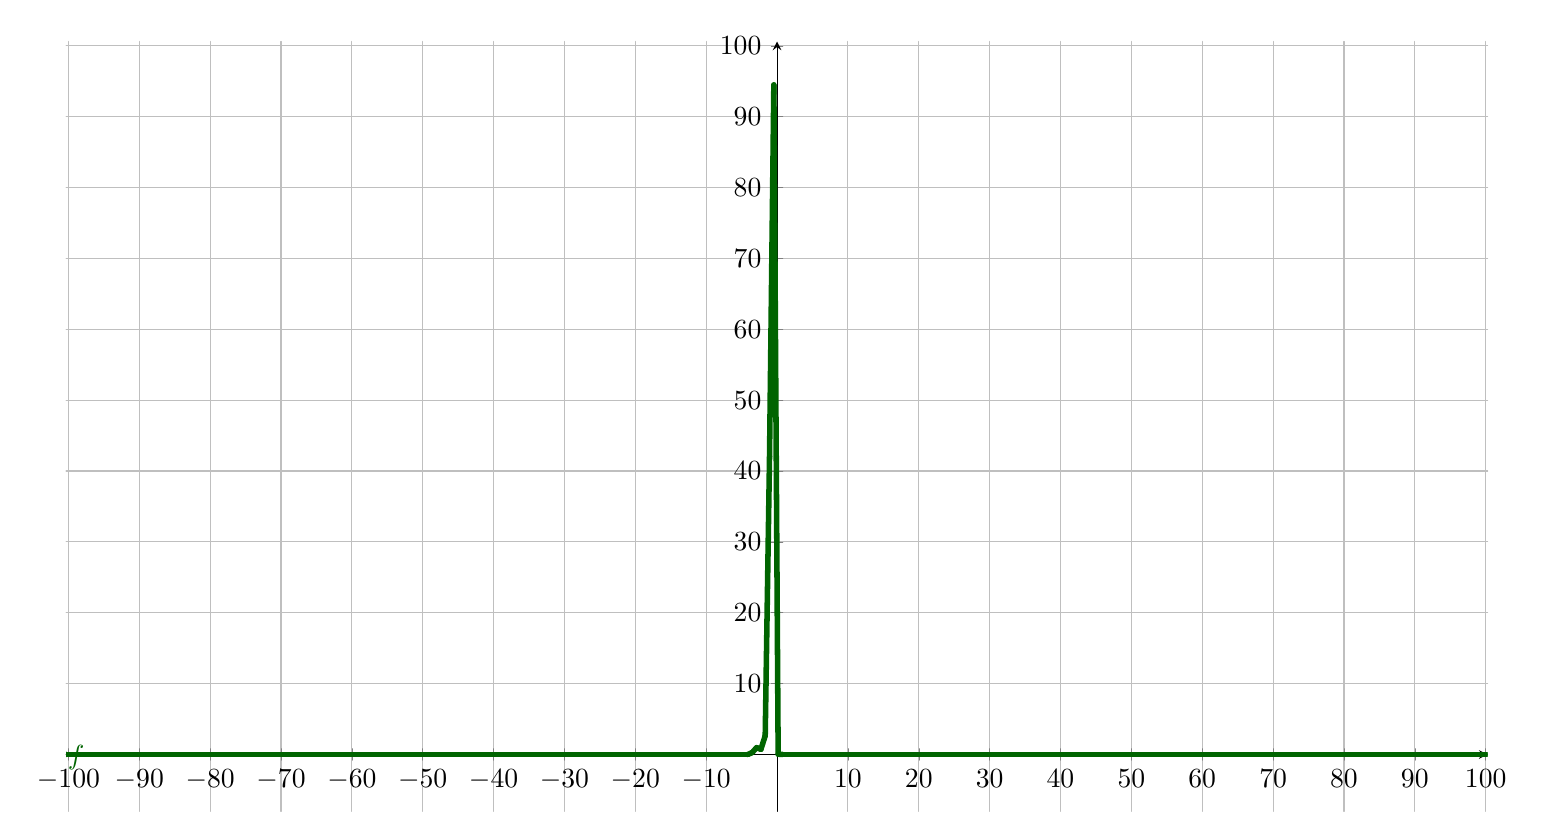
\begin{tikzpicture}[line cap=round,line join=round,>=triangle 45,x=0.09cm,y=0.09cm]
\begin{axis}[
x=0.09cm,y=0.09cm,
axis lines=middle,
ymajorgrids=true,
xmajorgrids=true,
xmin=-100.33083975787744,
xmax=100.27211796412013,
ymin=-8.041337462915347,
ymax=100.60446511729668,
xtick={-100,-90,...,100},
ytick={0,10,...,100},]
\clip(-100.33083975787744,-8.041337462915347) rectangle (143.27211796412013,151.60446511729668);
\draw[line width=2pt,color=qqwuqq] (-100.33083975787744,0) -- (-100.33083975787744,0);
\draw[line width=2pt,color=qqwuqq] (-100.33083975787744,0) -- (-99.72183236357245,0);
\draw[line width=2pt,color=qqwuqq] (-99.72183236357245,0) -- (-99.11282496926745,0);
\draw[line width=2pt,color=qqwuqq] (-99.11282496926745,0) -- (-98.50381757496245,0);
\draw[line width=2pt,color=qqwuqq] (-98.50381757496245,0) -- (-97.89481018065746,0);
\draw[line width=2pt,color=qqwuqq] (-97.89481018065746,0) -- (-97.28580278635246,0);
\draw[line width=2pt,color=qqwuqq] (-97.28580278635246,0) -- (-96.67679539204747,0);
\draw[line width=2pt,color=qqwuqq] (-96.67679539204747,0) -- (-96.06778799774247,0);
\draw[line width=2pt,color=qqwuqq] (-96.06778799774247,0) -- (-95.45878060343748,0);
\draw[line width=2pt,color=qqwuqq] (-95.45878060343748,0) -- (-94.84977320913248,0);
\draw[line width=2pt,color=qqwuqq] (-94.84977320913248,0) -- (-94.24076581482748,0);
\draw[line width=2pt,color=qqwuqq] (-94.24076581482748,0) -- (-93.63175842052249,0);
\draw[line width=2pt,color=qqwuqq] (-93.63175842052249,0) -- (-93.02275102621749,0);
\draw[line width=2pt,color=qqwuqq] (-93.02275102621749,0) -- (-92.4137436319125,0);
\draw[line width=2pt,color=qqwuqq] (-92.4137436319125,0) -- (-91.8047362376075,0);
\draw[line width=2pt,color=qqwuqq] (-91.8047362376075,0) -- (-91.1957288433025,0);
\draw[line width=2pt,color=qqwuqq] (-91.1957288433025,0) -- (-90.58672144899751,0);
\draw[line width=2pt,color=qqwuqq] (-90.58672144899751,0) -- (-89.97771405469251,0);
\draw[line width=2pt,color=qqwuqq] (-89.97771405469251,0) -- (-89.36870666038752,0);
\draw[line width=2pt,color=qqwuqq] (-89.36870666038752,0) -- (-88.75969926608252,0);
\draw[line width=2pt,color=qqwuqq] (-88.75969926608252,0) -- (-88.15069187177752,0);
\draw[line width=2pt,color=qqwuqq] (-88.15069187177752,0) -- (-87.54168447747253,0);
\draw[line width=2pt,color=qqwuqq] (-87.54168447747253,0) -- (-86.93267708316753,0);
\draw[line width=2pt,color=qqwuqq] (-86.93267708316753,0) -- (-86.32366968886254,0);
\draw[line width=2pt,color=qqwuqq] (-86.32366968886254,0) -- (-85.71466229455754,0);
\draw[line width=2pt,color=qqwuqq] (-85.71466229455754,0) -- (-85.10565490025255,0);
\draw[line width=2pt,color=qqwuqq] (-85.10565490025255,0) -- (-84.49664750594755,0);
\draw[line width=2pt,color=qqwuqq] (-84.49664750594755,0) -- (-83.88764011164255,0);
\draw[line width=2pt,color=qqwuqq] (-83.88764011164255,0) -- (-83.27863271733756,0);
\draw[line width=2pt,color=qqwuqq] (-83.27863271733756,0) -- (-82.66962532303256,0);
\draw[line width=2pt,color=qqwuqq] (-82.66962532303256,0) -- (-82.06061792872757,0);
\draw[line width=2pt,color=qqwuqq] (-82.06061792872757,0) -- (-81.45161053442257,0);
\draw[line width=2pt,color=qqwuqq] (-81.45161053442257,0) -- (-80.84260314011757,0);
\draw[line width=2pt,color=qqwuqq] (-80.84260314011757,0) -- (-80.23359574581258,0);
\draw[line width=2pt,color=qqwuqq] (-80.23359574581258,0) -- (-79.62458835150758,0);
\draw[line width=2pt,color=qqwuqq] (-79.62458835150758,0) -- (-79.01558095720259,0);
\draw[line width=2pt,color=qqwuqq] (-79.01558095720259,0) -- (-78.40657356289759,0);
\draw[line width=2pt,color=qqwuqq] (-78.40657356289759,0) -- (-77.7975661685926,0);
\draw[line width=2pt,color=qqwuqq] (-77.7975661685926,0) -- (-77.1885587742876,0);
\draw[line width=2pt,color=qqwuqq] (-77.1885587742876,0) -- (-76.5795513799826,0);
\draw[line width=2pt,color=qqwuqq] (-76.5795513799826,0) -- (-75.97054398567761,0);
\draw[line width=2pt,color=qqwuqq] (-75.97054398567761,0) -- (-75.36153659137261,0);
\draw[line width=2pt,color=qqwuqq] (-75.36153659137261,0) -- (-74.75252919706762,0);
\draw[line width=2pt,color=qqwuqq] (-74.75252919706762,0) -- (-74.14352180276262,0);
\draw[line width=2pt,color=qqwuqq] (-74.14352180276262,0) -- (-73.53451440845762,0);
\draw[line width=2pt,color=qqwuqq] (-73.53451440845762,0) -- (-72.92550701415263,0);
\draw[line width=2pt,color=qqwuqq] (-72.92550701415263,0) -- (-72.31649961984763,0);
\draw[line width=2pt,color=qqwuqq] (-72.31649961984763,0) -- (-71.70749222554264,0);
\draw[line width=2pt,color=qqwuqq] (-71.70749222554264,0) -- (-71.09848483123764,0);
\draw[line width=2pt,color=qqwuqq] (-71.09848483123764,0) -- (-70.48947743693265,0);
\draw[line width=2pt,color=qqwuqq] (-70.48947743693265,0) -- (-69.88047004262765,0);
\draw[line width=2pt,color=qqwuqq] (-69.88047004262765,0) -- (-69.27146264832265,0);
\draw[line width=2pt,color=qqwuqq] (-69.27146264832265,0) -- (-68.66245525401766,0);
\draw[line width=2pt,color=qqwuqq] (-68.66245525401766,0) -- (-68.05344785971266,0);
\draw[line width=2pt,color=qqwuqq] (-68.05344785971266,0) -- (-67.44444046540767,0);
\draw[line width=2pt,color=qqwuqq] (-67.44444046540767,0) -- (-66.83543307110267,0);
\draw[line width=2pt,color=qqwuqq] (-66.83543307110267,0) -- (-66.22642567679767,0);
\draw[line width=2pt,color=qqwuqq] (-66.22642567679767,0) -- (-65.61741828249268,0);
\draw[line width=2pt,color=qqwuqq] (-65.61741828249268,0) -- (-65.00841088818768,0);
\draw[line width=2pt,color=qqwuqq] (-65.00841088818768,0) -- (-64.39940349388269,0);
\draw[line width=2pt,color=qqwuqq] (-64.39940349388269,0) -- (-63.79039609957769,0);
\draw[line width=2pt,color=qqwuqq] (-63.79039609957769,0) -- (-63.181388705272695,0);
\draw[line width=2pt,color=qqwuqq] (-63.181388705272695,0) -- (-62.5723813109677,0);
\draw[line width=2pt,color=qqwuqq] (-62.5723813109677,0) -- (-61.963373916662704,0);
\draw[line width=2pt,color=qqwuqq] (-61.963373916662704,0) -- (-61.35436652235771,0);
\draw[line width=2pt,color=qqwuqq] (-61.35436652235771,0) -- (-60.74535912805271,0);
\draw[line width=2pt,color=qqwuqq] (-60.74535912805271,0) -- (-60.136351733747716,0);
\draw[line width=2pt,color=qqwuqq] (-60.136351733747716,0) -- (-59.52734433944272,0);
\draw[line width=2pt,color=qqwuqq] (-59.52734433944272,0) -- (-58.918336945137725,0);
\draw[line width=2pt,color=qqwuqq] (-58.918336945137725,0) -- (-58.30932955083273,0);
\draw[line width=2pt,color=qqwuqq] (-58.30932955083273,0) -- (-57.70032215652773,0);
\draw[line width=2pt,color=qqwuqq] (-57.70032215652773,0) -- (-57.09131476222274,0);
\draw[line width=2pt,color=qqwuqq] (-57.09131476222274,0) -- (-56.48230736791774,0);
\draw[line width=2pt,color=qqwuqq] (-56.48230736791774,0) -- (-55.873299973612745,0);
\draw[line width=2pt,color=qqwuqq] (-55.873299973612745,0) -- (-55.26429257930775,0);
\draw[line width=2pt,color=qqwuqq] (-55.26429257930775,0) -- (-54.655285185002754,0);
\draw[line width=2pt,color=qqwuqq] (-54.655285185002754,0) -- (-54.04627779069776,0);
\draw[line width=2pt,color=qqwuqq] (-54.04627779069776,0) -- (-53.43727039639276,0);
\draw[line width=2pt,color=qqwuqq] (-53.43727039639276,0) -- (-52.828263002087766,0);
\draw[line width=2pt,color=qqwuqq] (-52.828263002087766,0) -- (-52.21925560778277,0);
\draw[line width=2pt,color=qqwuqq] (-52.21925560778277,0) -- (-51.610248213477774,0);
\draw[line width=2pt,color=qqwuqq] (-51.610248213477774,0) -- (-51.00124081917278,0);
\draw[line width=2pt,color=qqwuqq] (-51.00124081917278,0) -- (-50.39223342486778,0);
\draw[line width=2pt,color=qqwuqq] (-50.39223342486778,0) -- (-49.78322603056279,0);
\draw[line width=2pt,color=qqwuqq] (-49.78322603056279,0) -- (-49.17421863625779,0);
\draw[line width=2pt,color=qqwuqq] (-49.17421863625779,0) -- (-48.565211241952795,0);
\draw[line width=2pt,color=qqwuqq] (-48.565211241952795,0) -- (-47.9562038476478,0);
\draw[line width=2pt,color=qqwuqq] (-47.9562038476478,0) -- (-47.347196453342804,0);
\draw[line width=2pt,color=qqwuqq] (-47.347196453342804,0) -- (-46.73818905903781,0);
\draw[line width=2pt,color=qqwuqq] (-46.73818905903781,0) -- (-46.12918166473281,0);
\draw[line width=2pt,color=qqwuqq] (-46.12918166473281,0) -- (-45.520174270427816,0);
\draw[line width=2pt,color=qqwuqq] (-45.520174270427816,0) -- (-44.91116687612282,0);
\draw[line width=2pt,color=qqwuqq] (-44.91116687612282,0) -- (-44.302159481817824,0);
\draw[line width=2pt,color=qqwuqq] (-44.302159481817824,0) -- (-43.69315208751283,0);
\draw[line width=2pt,color=qqwuqq] (-43.69315208751283,0) -- (-43.08414469320783,0);
\draw[line width=2pt,color=qqwuqq] (-43.08414469320783,0) -- (-42.47513729890284,0);
\draw[line width=2pt,color=qqwuqq] (-42.47513729890284,0) -- (-41.86612990459784,0);
\draw[line width=2pt,color=qqwuqq] (-41.86612990459784,0) -- (-41.257122510292845,0);
\draw[line width=2pt,color=qqwuqq] (-41.257122510292845,0) -- (-40.64811511598785,0);
\draw[line width=2pt,color=qqwuqq] (-40.64811511598785,0) -- (-40.03910772168285,0);
\draw[line width=2pt,color=qqwuqq] (-40.03910772168285,0) -- (-39.43010032737786,0);
\draw[line width=2pt,color=qqwuqq] (-39.43010032737786,0) -- (-38.82109293307286,0);
\draw[line width=2pt,color=qqwuqq] (-38.82109293307286,0) -- (-38.212085538767866,0);
\draw[line width=2pt,color=qqwuqq] (-38.212085538767866,0) -- (-37.60307814446287,0);
\draw[line width=2pt,color=qqwuqq] (-37.60307814446287,0) -- (-36.994070750157874,0);
\draw[line width=2pt,color=qqwuqq] (-36.994070750157874,0) -- (-36.38506335585288,0);
\draw[line width=2pt,color=qqwuqq] (-36.38506335585288,0) -- (-35.77605596154788,0);
\draw[line width=2pt,color=qqwuqq] (-35.77605596154788,0) -- (-35.16704856724289,0);
\draw[line width=2pt,color=qqwuqq] (-35.16704856724289,0) -- (-34.55804117293789,0);
\draw[line width=2pt,color=qqwuqq] (-34.55804117293789,0) -- (-33.949033778632895,0);
\draw[line width=2pt,color=qqwuqq] (-33.949033778632895,0) -- (-33.3400263843279,0);
\draw[line width=2pt,color=qqwuqq] (-33.3400263843279,0) -- (-32.7310189900229,0);
\draw[line width=2pt,color=qqwuqq] (-32.7310189900229,0) -- (-32.12201159571791,0);
\draw[line width=2pt,color=qqwuqq] (-32.12201159571791,0) -- (-31.513004201412915,0);
\draw[line width=2pt,color=qqwuqq] (-31.513004201412915,0) -- (-30.903996807107923,0);
\draw[line width=2pt,color=qqwuqq] (-30.903996807107923,0) -- (-30.29498941280293,0);
\draw[line width=2pt,color=qqwuqq] (-30.29498941280293,0) -- (-29.68598201849794,0);
\draw[line width=2pt,color=qqwuqq] (-29.68598201849794,0) -- (-29.076974624192946,0);
\draw[line width=2pt,color=qqwuqq] (-29.076974624192946,0) -- (-28.467967229887954,0);
\draw[line width=2pt,color=qqwuqq] (-28.467967229887954,0) -- (-27.85895983558296,0);
\draw[line width=2pt,color=qqwuqq] (-27.85895983558296,0) -- (-27.24995244127797,0);
\draw[line width=2pt,color=qqwuqq] (-27.24995244127797,0) -- (-26.640945046972977,0);
\draw[line width=2pt,color=qqwuqq] (-26.640945046972977,0) -- (-26.031937652667985,0);
\draw[line width=2pt,color=qqwuqq] (-26.031937652667985,0) -- (-25.422930258362992,0);
\draw[line width=2pt,color=qqwuqq] (-25.422930258362992,0) -- (-24.813922864058,0);
\draw[line width=2pt,color=qqwuqq] (-24.813922864058,0) -- (-24.204915469753008,0);
\draw[line width=2pt,color=qqwuqq] (-24.204915469753008,0) -- (-23.595908075448015,0);
\draw[line width=2pt,color=qqwuqq] (-23.595908075448015,0) -- (-22.986900681143023,0);
\draw[line width=2pt,color=qqwuqq] (-22.986900681143023,0) -- (-22.37789328683803,0);
\draw[line width=2pt,color=qqwuqq] (-22.37789328683803,0) -- (-21.76888589253304,0);
\draw[line width=2pt,color=qqwuqq] (-21.76888589253304,0) -- (-21.159878498228046,0);
\draw[line width=2pt,color=qqwuqq] (-21.159878498228046,0) -- (-20.550871103923054,0);
\draw[line width=2pt,color=qqwuqq] (-20.550871103923054,0) -- (-19.94186370961806,0);
\draw[line width=2pt,color=qqwuqq] (-19.94186370961806,0) -- (-19.33285631531307,0);
\draw[line width=2pt,color=qqwuqq] (-19.33285631531307,0) -- (-18.723848921008077,0);
\draw[line width=2pt,color=qqwuqq] (-18.723848921008077,0) -- (-18.114841526703085,0);
\draw[line width=2pt,color=qqwuqq] (-18.114841526703085,0) -- (-17.505834132398093,0);
\draw[line width=2pt,color=qqwuqq] (-17.505834132398093,0) -- (-16.8968267380931,0);
\draw[line width=2pt,color=qqwuqq] (-16.8968267380931,0) -- (-16.287819343788108,0);
\draw[line width=2pt,color=qqwuqq] (-16.287819343788108,0) -- (-15.678811949483114,0);
\draw[line width=2pt,color=qqwuqq] (-15.678811949483114,0) -- (-15.06980455517812,0);
\draw[line width=2pt,color=qqwuqq] (-15.06980455517812,0) -- (-14.460797160873126,0);
\draw[line width=2pt,color=qqwuqq] (-14.460797160873126,0) -- (-13.851789766568132,0);
\draw[line width=2pt,color=qqwuqq] (-13.851789766568132,0) -- (-13.242782372263138,0);
\draw[line width=2pt,color=qqwuqq] (-13.242782372263138,0) -- (-12.633774977958144,0);
\draw[line width=2pt,color=qqwuqq] (-12.633774977958144,0) -- (-12.02476758365315,0);
\draw[line width=2pt,color=qqwuqq] (-12.02476758365315,0) -- (-11.415760189348156,0);
\draw[line width=2pt,color=qqwuqq] (-11.415760189348156,0) -- (-10.806752795043161,0);
\draw[line width=2pt,color=qqwuqq] (-10.806752795043161,0) -- (-10.197745400738167,0);
\draw[line width=2pt,color=qqwuqq] (-10.197745400738167,0) -- (-9.588738006433173,0);
\draw[line width=2pt,color=qqwuqq] (-9.588738006433173,0) -- (-8.97973061212818,0);
\draw[line width=2pt,color=qqwuqq] (-8.97973061212818,0) -- (-8.370723217823185,0);
\draw[line width=2pt,color=qqwuqq] (-8.370723217823185,0) -- (-7.761715823518191,0);
\draw[line width=2pt,color=qqwuqq] (-7.761715823518191,0) -- (-7.152708429213197,0);
\draw[line width=2pt,color=qqwuqq] (-7.152708429213197,0) -- (-6.543701034908203,0);
\draw[line width=2pt,color=qqwuqq] (-6.543701034908203,0) -- (-5.934693640603209,0);
\draw[line width=2pt,color=qqwuqq] (-5.934693640603209,0) -- (-5.325686246298215,0);
\draw[line width=2pt,color=qqwuqq] (-5.325686246298215,0) -- (-4.716678851993221,0);
\draw[line width=2pt,color=qqwuqq] (-4.716678851993221,0) -- (-4.107671457688227,0);
\draw[line width=2pt,color=qqwuqq] (-4.107671457688227,0) -- (-3.4986640633832327,0.2714885978611352);
\draw[line width=2pt,color=qqwuqq] (-3.4986640633832327,0.2714885978611352) -- (-2.8896566690782386,0.9691836196328023);
\draw[line width=2pt,color=qqwuqq] (-2.8896566690782386,0.9691836196328023) -- (-2.2806492747732445,0.7180541654879805);
\draw[line width=2pt,color=qqwuqq] (-2.2806492747732445,0.7180541654879805) -- (-1.6716418804682505,2.634118140661137);
\draw[line width=2pt,color=qqwuqq] (-1.6716418804682505,2.634118140661137) -- (-1.0626344861632564,42.0416296000723);
\draw[line width=2pt,color=qqwuqq] (-1.0626344861632564,42.0416296000723) -- (-0.45362709185826244,94.47970797764486);
\draw[line width=2pt,color=qqwuqq] (-0.45362709185826244,94.47970797764486) -- (0.1553803024467315,0.035634430581235);
\draw[line width=2pt,color=qqwuqq] (0.1553803024467315,0.035634430581235) -- (0.7643876967517255,0);
\draw[line width=2pt,color=qqwuqq] (0.7643876967517255,0) -- (1.3733950910567194,0);
\draw[line width=2pt,color=qqwuqq] (1.3733950910567194,0) -- (1.9824024853617135,0);
\draw[line width=2pt,color=qqwuqq] (1.9824024853617135,0) -- (2.5914098796667075,0);
\draw[line width=2pt,color=qqwuqq] (2.5914098796667075,0) -- (3.2004172739717016,0);
\draw[line width=2pt,color=qqwuqq] (3.2004172739717016,0) -- (3.8094246682766957,0);
\draw[line width=2pt,color=qqwuqq] (3.8094246682766957,0) -- (4.418432062581689,0);
\draw[line width=2pt,color=qqwuqq] (4.418432062581689,0) -- (5.027439456886683,0);
\draw[line width=2pt,color=qqwuqq] (5.027439456886683,0) -- (5.636446851191677,0);
\draw[line width=2pt,color=qqwuqq] (5.636446851191677,0) -- (6.2454542454966715,0);
\draw[line width=2pt,color=qqwuqq] (6.2454542454966715,0) -- (6.854461639801666,0);
\draw[line width=2pt,color=qqwuqq] (6.854461639801666,0) -- (7.46346903410666,0);
\draw[line width=2pt,color=qqwuqq] (7.46346903410666,0) -- (8.072476428411653,0);
\draw[line width=2pt,color=qqwuqq] (8.072476428411653,0) -- (8.681483822716647,0);
\draw[line width=2pt,color=qqwuqq] (8.681483822716647,0) -- (9.290491217021641,0);
\draw[line width=2pt,color=qqwuqq] (9.290491217021641,0) -- (9.899498611326635,0);
\draw[line width=2pt,color=qqwuqq] (9.899498611326635,0) -- (10.508506005631629,0);
\draw[line width=2pt,color=qqwuqq] (10.508506005631629,0) -- (11.117513399936623,0);
\draw[line width=2pt,color=qqwuqq] (11.117513399936623,0) -- (11.726520794241617,0);
\draw[line width=2pt,color=qqwuqq] (11.726520794241617,0) -- (12.335528188546611,0);
\draw[line width=2pt,color=qqwuqq] (12.335528188546611,0) -- (12.944535582851605,0);
\draw[line width=2pt,color=qqwuqq] (12.944535582851605,0) -- (13.5535429771566,0);
\draw[line width=2pt,color=qqwuqq] (13.5535429771566,0) -- (14.162550371461593,0);
\draw[line width=2pt,color=qqwuqq] (14.162550371461593,0) -- (14.771557765766588,0);
\draw[line width=2pt,color=qqwuqq] (14.771557765766588,0) -- (15.380565160071582,0);
\draw[line width=2pt,color=qqwuqq] (15.380565160071582,0) -- (15.989572554376576,0);
\draw[line width=2pt,color=qqwuqq] (15.989572554376576,0) -- (16.598579948681568,0);
\draw[line width=2pt,color=qqwuqq] (16.598579948681568,0) -- (17.20758734298656,0);
\draw[line width=2pt,color=qqwuqq] (17.20758734298656,0) -- (17.816594737291553,0);
\draw[line width=2pt,color=qqwuqq] (17.816594737291553,0) -- (18.425602131596545,0);
\draw[line width=2pt,color=qqwuqq] (18.425602131596545,0) -- (19.034609525901537,0);
\draw[line width=2pt,color=qqwuqq] (19.034609525901537,0) -- (19.64361692020653,0);
\draw[line width=2pt,color=qqwuqq] (19.64361692020653,0) -- (20.25262431451152,0);
\draw[line width=2pt,color=qqwuqq] (20.25262431451152,0) -- (20.861631708816514,0);
\draw[line width=2pt,color=qqwuqq] (20.861631708816514,0) -- (21.470639103121506,0);
\draw[line width=2pt,color=qqwuqq] (21.470639103121506,0) -- (22.0796464974265,0);
\draw[line width=2pt,color=qqwuqq] (22.0796464974265,0) -- (22.68865389173149,0);
\draw[line width=2pt,color=qqwuqq] (22.68865389173149,0) -- (23.297661286036483,0);
\draw[line width=2pt,color=qqwuqq] (23.297661286036483,0) -- (23.906668680341475,0);
\draw[line width=2pt,color=qqwuqq] (23.906668680341475,0) -- (24.515676074646468,0);
\draw[line width=2pt,color=qqwuqq] (24.515676074646468,0) -- (25.12468346895146,0);
\draw[line width=2pt,color=qqwuqq] (25.12468346895146,0) -- (25.733690863256452,0);
\draw[line width=2pt,color=qqwuqq] (25.733690863256452,0) -- (26.342698257561445,0);
\draw[line width=2pt,color=qqwuqq] (26.342698257561445,0) -- (26.951705651866437,0);
\draw[line width=2pt,color=qqwuqq] (26.951705651866437,0) -- (27.56071304617143,0);
\draw[line width=2pt,color=qqwuqq] (27.56071304617143,0) -- (28.16972044047642,0);
\draw[line width=2pt,color=qqwuqq] (28.16972044047642,0) -- (28.778727834781414,0);
\draw[line width=2pt,color=qqwuqq] (28.778727834781414,0) -- (29.387735229086406,0);
\draw[line width=2pt,color=qqwuqq] (29.387735229086406,0) -- (29.9967426233914,0);
\draw[line width=2pt,color=qqwuqq] (29.9967426233914,0) -- (30.60575001769639,0);
\draw[line width=2pt,color=qqwuqq] (30.60575001769639,0) -- (31.214757412001383,0);
\draw[line width=2pt,color=qqwuqq] (31.214757412001383,0) -- (31.823764806306375,0);
\draw[line width=2pt,color=qqwuqq] (31.823764806306375,0) -- (32.43277220061137,0);
\draw[line width=2pt,color=qqwuqq] (32.43277220061137,0) -- (33.04177959491636,0);
\draw[line width=2pt,color=qqwuqq] (33.04177959491636,0) -- (33.65078698922136,0);
\draw[line width=2pt,color=qqwuqq] (33.65078698922136,0) -- (34.259794383526355,0);
\draw[line width=2pt,color=qqwuqq] (34.259794383526355,0) -- (34.86880177783135,0);
\draw[line width=2pt,color=qqwuqq] (34.86880177783135,0) -- (35.47780917213635,0);
\draw[line width=2pt,color=qqwuqq] (35.47780917213635,0) -- (36.08681656644134,0);
\draw[line width=2pt,color=qqwuqq] (36.08681656644134,0) -- (36.69582396074634,0);
\draw[line width=2pt,color=qqwuqq] (36.69582396074634,0) -- (37.304831355051334,0);
\draw[line width=2pt,color=qqwuqq] (37.304831355051334,0) -- (37.91383874935633,0);
\draw[line width=2pt,color=qqwuqq] (37.91383874935633,0) -- (38.522846143661326,0);
\draw[line width=2pt,color=qqwuqq] (38.522846143661326,0) -- (39.13185353796632,0);
\draw[line width=2pt,color=qqwuqq] (39.13185353796632,0) -- (39.74086093227132,0);
\draw[line width=2pt,color=qqwuqq] (39.74086093227132,0) -- (40.34986832657631,0);
\draw[line width=2pt,color=qqwuqq] (40.34986832657631,0) -- (40.95887572088131,0);
\draw[line width=2pt,color=qqwuqq] (40.95887572088131,0) -- (41.567883115186305,0);
\draw[line width=2pt,color=qqwuqq] (41.567883115186305,0) -- (42.1768905094913,0);
\draw[line width=2pt,color=qqwuqq] (42.1768905094913,0) -- (42.7858979037963,0);
\draw[line width=2pt,color=qqwuqq] (42.7858979037963,0) -- (43.39490529810129,0);
\draw[line width=2pt,color=qqwuqq] (43.39490529810129,0) -- (44.00391269240629,0);
\draw[line width=2pt,color=qqwuqq] (44.00391269240629,0) -- (44.612920086711284,0);
\draw[line width=2pt,color=qqwuqq] (44.612920086711284,0) -- (45.22192748101628,0);
\draw[line width=2pt,color=qqwuqq] (45.22192748101628,0) -- (45.830934875321276,0);
\draw[line width=2pt,color=qqwuqq] (45.830934875321276,0) -- (46.43994226962627,0);
\draw[line width=2pt,color=qqwuqq] (46.43994226962627,0) -- (47.04894966393127,0);
\draw[line width=2pt,color=qqwuqq] (47.04894966393127,0) -- (47.65795705823626,0);
\draw[line width=2pt,color=qqwuqq] (47.65795705823626,0) -- (48.26696445254126,0);
\draw[line width=2pt,color=qqwuqq] (48.26696445254126,0) -- (48.875971846846255,0);
\draw[line width=2pt,color=qqwuqq] (48.875971846846255,0) -- (49.48497924115125,0);
\draw[line width=2pt,color=qqwuqq] (49.48497924115125,0) -- (50.09398663545625,0);
\draw[line width=2pt,color=qqwuqq] (50.09398663545625,0) -- (50.70299402976124,0);
\draw[line width=2pt,color=qqwuqq] (50.70299402976124,0) -- (51.31200142406624,0);
\draw[line width=2pt,color=qqwuqq] (51.31200142406624,0) -- (51.921008818371234,0);
\draw[line width=2pt,color=qqwuqq] (51.921008818371234,0) -- (52.53001621267623,0);
\draw[line width=2pt,color=qqwuqq] (52.53001621267623,0) -- (53.139023606981226,0);
\draw[line width=2pt,color=qqwuqq] (53.139023606981226,0) -- (53.74803100128622,0);
\draw[line width=2pt,color=qqwuqq] (53.74803100128622,0) -- (54.35703839559122,0);
\draw[line width=2pt,color=qqwuqq] (54.35703839559122,0) -- (54.966045789896214,0);
\draw[line width=2pt,color=qqwuqq] (54.966045789896214,0) -- (55.57505318420121,0);
\draw[line width=2pt,color=qqwuqq] (55.57505318420121,0) -- (56.184060578506205,0);
\draw[line width=2pt,color=qqwuqq] (56.184060578506205,0) -- (56.7930679728112,0);
\draw[line width=2pt,color=qqwuqq] (56.7930679728112,0) -- (57.4020753671162,0);
\draw[line width=2pt,color=qqwuqq] (57.4020753671162,0) -- (58.01108276142119,0);
\draw[line width=2pt,color=qqwuqq] (58.01108276142119,0) -- (58.62009015572619,0);
\draw[line width=2pt,color=qqwuqq] (58.62009015572619,0) -- (59.229097550031184,0);
\draw[line width=2pt,color=qqwuqq] (59.229097550031184,0) -- (59.83810494433618,0);
\draw[line width=2pt,color=qqwuqq] (59.83810494433618,0) -- (60.447112338641176,0);
\draw[line width=2pt,color=qqwuqq] (60.447112338641176,0) -- (61.05611973294617,0);
\draw[line width=2pt,color=qqwuqq] (61.05611973294617,0) -- (61.66512712725117,0);
\draw[line width=2pt,color=qqwuqq] (61.66512712725117,0) -- (62.274134521556164,0);
\draw[line width=2pt,color=qqwuqq] (62.274134521556164,0) -- (62.88314191586116,0);
\draw[line width=2pt,color=qqwuqq] (62.88314191586116,0) -- (63.492149310166155,0);
\draw[line width=2pt,color=qqwuqq] (63.492149310166155,0) -- (64.10115670447115,0);
\draw[line width=2pt,color=qqwuqq] (64.10115670447115,0) -- (64.71016409877615,0);
\draw[line width=2pt,color=qqwuqq] (64.71016409877615,0) -- (65.31917149308114,0);
\draw[line width=2pt,color=qqwuqq] (65.31917149308114,0) -- (65.92817888738614,0);
\draw[line width=2pt,color=qqwuqq] (65.92817888738614,0) -- (66.53718628169113,0);
\draw[line width=2pt,color=qqwuqq] (66.53718628169113,0) -- (67.14619367599613,0);
\draw[line width=2pt,color=qqwuqq] (67.14619367599613,0) -- (67.75520107030113,0);
\draw[line width=2pt,color=qqwuqq] (67.75520107030113,0) -- (68.36420846460612,0);
\draw[line width=2pt,color=qqwuqq] (68.36420846460612,0) -- (68.97321585891112,0);
\draw[line width=2pt,color=qqwuqq] (68.97321585891112,0) -- (69.58222325321611,0);
\draw[line width=2pt,color=qqwuqq] (69.58222325321611,0) -- (70.19123064752111,0);
\draw[line width=2pt,color=qqwuqq] (70.19123064752111,0) -- (70.8002380418261,0);
\draw[line width=2pt,color=qqwuqq] (70.8002380418261,0) -- (71.4092454361311,0);
\draw[line width=2pt,color=qqwuqq] (71.4092454361311,0) -- (72.0182528304361,0);
\draw[line width=2pt,color=qqwuqq] (72.0182528304361,0) -- (72.6272602247411,0);
\draw[line width=2pt,color=qqwuqq] (72.6272602247411,0) -- (73.23626761904609,0);
\draw[line width=2pt,color=qqwuqq] (73.23626761904609,0) -- (73.84527501335108,0);
\draw[line width=2pt,color=qqwuqq] (73.84527501335108,0) -- (74.45428240765608,0);
\draw[line width=2pt,color=qqwuqq] (74.45428240765608,0) -- (75.06328980196108,0);
\draw[line width=2pt,color=qqwuqq] (75.06328980196108,0) -- (75.67229719626607,0);
\draw[line width=2pt,color=qqwuqq] (75.67229719626607,0) -- (76.28130459057107,0);
\draw[line width=2pt,color=qqwuqq] (76.28130459057107,0) -- (76.89031198487606,0);
\draw[line width=2pt,color=qqwuqq] (76.89031198487606,0) -- (77.49931937918106,0);
\draw[line width=2pt,color=qqwuqq] (77.49931937918106,0) -- (78.10832677348606,0);
\draw[line width=2pt,color=qqwuqq] (78.10832677348606,0) -- (78.71733416779105,0);
\draw[line width=2pt,color=qqwuqq] (78.71733416779105,0) -- (79.32634156209605,0);
\draw[line width=2pt,color=qqwuqq] (79.32634156209605,0) -- (79.93534895640104,0);
\draw[line width=2pt,color=qqwuqq] (79.93534895640104,0) -- (80.54435635070604,0);
\draw[line width=2pt,color=qqwuqq] (80.54435635070604,0) -- (81.15336374501103,0);
\draw[line width=2pt,color=qqwuqq] (81.15336374501103,0) -- (81.76237113931603,0);
\draw[line width=2pt,color=qqwuqq] (81.76237113931603,0) -- (82.37137853362103,0);
\draw[line width=2pt,color=qqwuqq] (82.37137853362103,0) -- (82.98038592792602,0);
\draw[line width=2pt,color=qqwuqq] (82.98038592792602,0) -- (83.58939332223102,0);
\draw[line width=2pt,color=qqwuqq] (83.58939332223102,0) -- (84.19840071653601,0);
\draw[line width=2pt,color=qqwuqq] (84.19840071653601,0) -- (84.80740811084101,0);
\draw[line width=2pt,color=qqwuqq] (84.80740811084101,0) -- (85.416415505146,0);
\draw[line width=2pt,color=qqwuqq] (85.416415505146,0) -- (86.025422899451,0);
\draw[line width=2pt,color=qqwuqq] (86.025422899451,0) -- (86.634430293756,0);
\draw[line width=2pt,color=qqwuqq] (86.634430293756,0) -- (87.243437688061,0);
\draw[line width=2pt,color=qqwuqq] (87.243437688061,0) -- (87.85244508236599,0);
\draw[line width=2pt,color=qqwuqq] (87.85244508236599,0) -- (88.46145247667098,0);
\draw[line width=2pt,color=qqwuqq] (88.46145247667098,0) -- (89.07045987097598,0);
\draw[line width=2pt,color=qqwuqq] (89.07045987097598,0) -- (89.67946726528098,0);
\draw[line width=2pt,color=qqwuqq] (89.67946726528098,0) -- (90.28847465958597,0);
\draw[line width=2pt,color=qqwuqq] (90.28847465958597,0) -- (90.89748205389097,0);
\draw[line width=2pt,color=qqwuqq] (90.89748205389097,0) -- (91.50648944819596,0);
\draw[line width=2pt,color=qqwuqq] (91.50648944819596,0) -- (92.11549684250096,0);
\draw[line width=2pt,color=qqwuqq] (92.11549684250096,0) -- (92.72450423680596,0);
\draw[line width=2pt,color=qqwuqq] (92.72450423680596,0) -- (93.33351163111095,0);
\draw[line width=2pt,color=qqwuqq] (93.33351163111095,0) -- (93.94251902541595,0);
\draw[line width=2pt,color=qqwuqq] (93.94251902541595,0) -- (94.55152641972094,0);
\draw[line width=2pt,color=qqwuqq] (94.55152641972094,0) -- (95.16053381402594,0);
\draw[line width=2pt,color=qqwuqq] (95.16053381402594,0) -- (95.76954120833093,0);
\draw[line width=2pt,color=qqwuqq] (95.76954120833093,0) -- (96.37854860263593,0);
\draw[line width=2pt,color=qqwuqq] (96.37854860263593,0) -- (96.98755599694093,0);
\draw[line width=2pt,color=qqwuqq] (96.98755599694093,0) -- (97.59656339124592,0);
\draw[line width=2pt,color=qqwuqq] (97.59656339124592,0) -- (98.20557078555092,0);
\draw[line width=2pt,color=qqwuqq] (98.20557078555092,0) -- (98.81457817985591,0);
\draw[line width=2pt,color=qqwuqq] (98.81457817985591,0) -- (99.42358557416091,0);
\draw[line width=2pt,color=qqwuqq] (99.42358557416091,0) -- (100.0325929684659,0);
\draw[line width=2pt,color=qqwuqq] (100.0325929684659,0) -- (100.6416003627709,0);
\draw[line width=2pt,color=qqwuqq] (100.6416003627709,0) -- (101.2506077570759,0);
\draw[line width=2pt,color=qqwuqq] (101.2506077570759,0) -- (101.8596151513809,0);
\draw[line width=2pt,color=qqwuqq] (101.8596151513809,0) -- (102.46862254568589,0);
\draw[line width=2pt,color=qqwuqq] (102.46862254568589,0) -- (103.07762993999089,0);
\draw[line width=2pt,color=qqwuqq] (103.07762993999089,0) -- (103.68663733429588,0);
\draw[line width=2pt,color=qqwuqq] (103.68663733429588,0) -- (104.29564472860088,0);
\draw[line width=2pt,color=qqwuqq] (104.29564472860088,0) -- (104.90465212290587,0);
\draw[line width=2pt,color=qqwuqq] (104.90465212290587,0) -- (105.51365951721087,0);
\draw[line width=2pt,color=qqwuqq] (105.51365951721087,0) -- (106.12266691151586,0);
\draw[line width=2pt,color=qqwuqq] (106.12266691151586,0) -- (106.73167430582086,0);
\draw[line width=2pt,color=qqwuqq] (106.73167430582086,0) -- (107.34068170012586,0);
\draw[line width=2pt,color=qqwuqq] (107.34068170012586,0) -- (107.94968909443085,0);
\draw[line width=2pt,color=qqwuqq] (107.94968909443085,0) -- (108.55869648873585,0);
\draw[line width=2pt,color=qqwuqq] (108.55869648873585,0) -- (109.16770388304084,0);
\draw[line width=2pt,color=qqwuqq] (109.16770388304084,0) -- (109.77671127734584,0);
\draw[line width=2pt,color=qqwuqq] (109.77671127734584,0) -- (110.38571867165084,0);
\draw[line width=2pt,color=qqwuqq] (110.38571867165084,0) -- (110.99472606595583,0);
\draw[line width=2pt,color=qqwuqq] (110.99472606595583,0) -- (111.60373346026083,0);
\draw[line width=2pt,color=qqwuqq] (111.60373346026083,0) -- (112.21274085456582,0);
\draw[line width=2pt,color=qqwuqq] (112.21274085456582,0) -- (112.82174824887082,0);
\draw[line width=2pt,color=qqwuqq] (112.82174824887082,0) -- (113.43075564317581,0);
\draw[line width=2pt,color=qqwuqq] (113.43075564317581,0) -- (114.03976303748081,0);
\draw[line width=2pt,color=qqwuqq] (114.03976303748081,0) -- (114.6487704317858,0);
\draw[line width=2pt,color=qqwuqq] (114.6487704317858,0) -- (115.2577778260908,0);
\draw[line width=2pt,color=qqwuqq] (115.2577778260908,0) -- (115.8667852203958,0);
\draw[line width=2pt,color=qqwuqq] (115.8667852203958,0) -- (116.4757926147008,0);
\draw[line width=2pt,color=qqwuqq] (116.4757926147008,0) -- (117.08480000900579,0);
\draw[line width=2pt,color=qqwuqq] (117.08480000900579,0) -- (117.69380740331079,0);
\draw[line width=2pt,color=qqwuqq] (117.69380740331079,0) -- (118.30281479761578,0);
\draw[line width=2pt,color=qqwuqq] (118.30281479761578,0) -- (118.91182219192078,0);
\draw[line width=2pt,color=qqwuqq] (118.91182219192078,0) -- (119.52082958622577,0);
\draw[line width=2pt,color=qqwuqq] (119.52082958622577,0) -- (120.12983698053077,0);
\draw[line width=2pt,color=qqwuqq] (120.12983698053077,0) -- (120.73884437483576,0);
\draw[line width=2pt,color=qqwuqq] (120.73884437483576,0) -- (121.34785176914076,0);
\draw[line width=2pt,color=qqwuqq] (121.34785176914076,0) -- (121.95685916344576,0);
\draw[line width=2pt,color=qqwuqq] (121.95685916344576,0) -- (122.56586655775075,0);
\draw[line width=2pt,color=qqwuqq] (122.56586655775075,0) -- (123.17487395205575,0);
\draw[line width=2pt,color=qqwuqq] (123.17487395205575,0) -- (123.78388134636074,0);
\draw[line width=2pt,color=qqwuqq] (123.78388134636074,0) -- (124.39288874066574,0);
\draw[line width=2pt,color=qqwuqq] (124.39288874066574,0) -- (125.00189613497074,0);
\draw[line width=2pt,color=qqwuqq] (125.00189613497074,0) -- (125.61090352927573,0);
\draw[line width=2pt,color=qqwuqq] (125.61090352927573,0) -- (126.21991092358073,0);
\draw[line width=2pt,color=qqwuqq] (126.21991092358073,0) -- (126.82891831788572,0);
\draw[line width=2pt,color=qqwuqq] (126.82891831788572,0) -- (127.43792571219072,0);
\draw[line width=2pt,color=qqwuqq] (127.43792571219072,0) -- (128.04693310649571,0);
\draw[line width=2pt,color=qqwuqq] (128.04693310649571,0) -- (128.6559405008007,0);
\draw[line width=2pt,color=qqwuqq] (128.6559405008007,0) -- (129.2649478951057,0);
\draw[line width=2pt,color=qqwuqq] (129.2649478951057,0) -- (129.8739552894107,0);
\draw[line width=2pt,color=qqwuqq] (129.8739552894107,0) -- (130.4829626837157,0);
\draw[line width=2pt,color=qqwuqq] (130.4829626837157,0) -- (131.0919700780207,0);
\draw[line width=2pt,color=qqwuqq] (131.0919700780207,0) -- (131.7009774723257,0);
\draw[line width=2pt,color=qqwuqq] (131.7009774723257,0) -- (132.30998486663069,0);
\draw[line width=2pt,color=qqwuqq] (132.30998486663069,0) -- (132.91899226093568,0);
\draw[line width=2pt,color=qqwuqq] (132.91899226093568,0) -- (133.52799965524068,0);
\draw[line width=2pt,color=qqwuqq] (133.52799965524068,0) -- (134.13700704954567,0);
\draw[line width=2pt,color=qqwuqq] (134.13700704954567,0) -- (134.74601444385067,0);
\draw[line width=2pt,color=qqwuqq] (134.74601444385067,0) -- (135.35502183815566,0);
\draw[line width=2pt,color=qqwuqq] (135.35502183815566,0) -- (135.96402923246066,0);
\draw[line width=2pt,color=qqwuqq] (135.96402923246066,0) -- (136.57303662676566,0);
\draw[line width=2pt,color=qqwuqq] (136.57303662676566,0) -- (137.18204402107065,0);
\draw[line width=2pt,color=qqwuqq] (137.18204402107065,0) -- (137.79105141537565,0);
\draw[line width=2pt,color=qqwuqq] (137.79105141537565,0) -- (138.40005880968064,0);
\draw[line width=2pt,color=qqwuqq] (138.40005880968064,0) -- (139.00906620398564,0);
\draw[line width=2pt,color=qqwuqq] (139.00906620398564,0) -- (139.61807359829064,0);
\draw[line width=2pt,color=qqwuqq] (139.61807359829064,0) -- (140.22708099259563,0);
\draw[line width=2pt,color=qqwuqq] (140.22708099259563,0) -- (140.83608838690063,0);
\draw[line width=2pt,color=qqwuqq] (140.83608838690063,0) -- (141.44509578120562,0);
\draw[line width=2pt,color=qqwuqq] (141.44509578120562,0) -- (142.05410317551062,0);
\draw[line width=2pt,color=qqwuqq] (142.05410317551062,0) -- (142.66311056981561,0);
\begin{scriptsize}
\draw[color=qqwuqq] (-98.89975188614247,-0.4883736954252371) node {$f$};
\end{scriptsize}
\end{axis}
\end{tikzpicture}

\i \textbf{(4).}
\begin{gather*}
    f(x) = e^x\sin3x;\\
    f\hatch(x) = (e^x)\hatch\sin3x + e^x(\sin3x)\hatch = \limit{x}{x_0} \frac{\sin3x(e^x-e^{x_0}) + 3e^x(\sin3x - \sin3x_0)}{x-x_0};\\
    \limit{x}{x_0} \frac{\sin3x(e^x-e^{x_0}) + 3e^x(\sin3x - \sin3x_0)}{x-x_0} = \limit{x}{x_0} \sin3x\frac{e^x - e^{x_0}}{x-x_0} + \limit{x}{x_0} 3e^x\frac{\sin3x - \sin3x_0}{x-x_0} = \\
    = \limit{x}{x_0}e^{x_0}\sin3x\frac{e^{x-x_0} - 1}{x-x_0} + \limit{x}{x_0} 3e^x\frac{\sin3x - \sin3x_0}{x-x_0} \sim \\
    \sim e^x\sin3x + 3e^x\limit{x}{x_0}\frac{\sin3x - \sin3x_0}{x-x_0} = e^x\sin3x + 3e^x\limit{x}{x_0}\frac{2\sin\frac{3x-3x_0}{2}\cos\frac{3x+3x_0}{2}}{x-x_0} \sim \\
    \sim e^x\sin3x + 3e^x\cos3x = e^x(\sin3x + 3\cos3x)
\end{gather*}

\i \textbf{(2).}
\begin{gather*}
    f(x) = 
    \begin{cases}
        x^4\cos(\frac{1}{x^2}), &x \ne 0,\\
        0, &x = 0.
    \end{cases}\\
    \text{При } x \ne 0: \quad f\hatch(x) = 4x^3\cos(\frac{1}{x^2}) + x^4(\cos(\frac{1}{x^2}))\hatch =\\
    = 4x^3\cos\frac{1}{x^2} - \sin\frac{1}{x^2}(\frac{1}{x^2})\hatch x^4 = 4x^3\cos\frac{1}{x^2} + 2x\sin\frac{1}{x^2}.
    \intertext{Легко убедиться, что полученная функция является непрерывной для всех $x\ne0$, так как она выражается как сумма и произведение непрерывных функций.
    Осталось только посчитать производную при $x=0$. Сделаем это по определению.}
    f\hatch(0) = \limit{x}{0}\frac{f(x) - 0}{x - 0} = \limit{x}{0} x^3\cos(\frac{1}{x^2}).
    \intertext{В силу того, что $\abs{\cos\frac{1}{x^2}} \leq 1$ верно, что}
    \limit{x}{0} x^3\cos(\frac{1}{x^2}) = 0.
\end{gather*}
Осталось определить, верно ли, что $\limit{x}{0} f\hatch(x) = 0:$
\begin{gather*}
    \limit{x}{0} 4x^3\cos\frac{1}{x^2} + 2x\sin\frac{1}{x^2} = \limit{x}{0} 2x(2x^2\cos\frac{1}{x^2}+\sin\frac{1}{x^2});
\end{gather*}
Тут мы можем аналогично ограничить часть в скобках "--- $\abs{2x^2\cos\frac{1}{x^2}+\sin\frac{1}{x^2}} \leq \abs{2x^2\cos\frac{1}{x^2}} + \abs{\sin\frac{1}{x^2}}$, а при $x \seek 0$ "--- $\abs{2x^2\cos\frac{1}{x^2}} + \abs{\sin\frac{1}{x^2}} \leq \abs{\cos\frac{1}{x^2}} + \abs{\sin\frac{1}{x^2}} \leq 2$. Следовательно $\limit{x}{0} f\hatch(x) = 0$.\\
Таким образом, из определение неприрывности по Гейне, производная $f(x)$ непрерывна при всех $\RR$.

\i \textbf{(1).}
\begin{gather*}
    y = \arccos\frac{1}{\sqrt{1+2x^2}};\\
    \frac{dy}{dx} = f\hatch(x) => dy = f\hatch(x) \cdot dx.\\
    \letus u = \frac{1}{\sqrt{1+2x^2}}:
    f\hatch(x) = \frac{d\arccos(u)}{du} \cdot \frac{du}{dx} = \frac{\frac{d}{dx}\brackets{\frac{1}{\sqrt{1+2x^2}}}}{\sqrt{1-\frac{1}{1+2x^2}}} = \\
    = -\frac{1}{\sqrt{1 - \frac{1}{1+2x^2}}}\brackets{-\frac{\frac{d}{dx}(1+2x^2)}{2(1+2x^2)^{3/2}}} = \frac{\frac{d}{dx}(1+2x^2)}{2(1+2x^2)^{3/2}\sqrt{1-\frac{1}{1+2x^2}}} = \\
    = \frac{\frac{d}{dx}1 + \frac{d}{dx}(2x^2)}{2(1+2x^2)^{3/2}\sqrt{1-\frac{1}{1+2x^2}}} = \frac{0 + 2x }{(1+2x^2)^{3/2}\sqrt{1-\frac{1}{1+2x^2}}} = \\
    = 2x\frac{1}{(1+2x)^{3/2}\sqrt{1 - \frac{1}{1+2x^2}}} => dy = 2x\frac{1}{(1+2x)^{3/2}\sqrt{1 - \frac{1}{1+2x^2}}} \cdot dx.
\end{gather*}

\i \textbf{(9).}
\begin{gather*}
    f(x) = \sqrt[4]{\frac{e^{\tg x}(x^4+1)}{x\cos x}}, \quad
    g(x) = (\cos x)^{\sqrt{x}}.
\end{gather*}
\pu
\begin{gather*}
    \frac{d}{dx}f(x) = \frac{d\sqrt[4]{\frac{(x^4+1)e^{\tg x}\sec x}{x}}}{d\frac{(x^4+1)e^{\tg x}\sec x}{x}} \cdot \frac{d\frac{(x^4+1)e^{\tg x}\sec x}{x}}{dx} = \\
     = \frac{\frac{d}{dx}\brackets{\frac{e^{\tg x}(x^4+1)\sec x}{x}}}{4\brackets{\frac{(x^4+1)e^{\tg x}\sec x}{x}}^{3/4}} = 
    \frac{1}{4\brackets{\frac{(x^4+1)e^{\tg x}\sec x}{x}}^{3/4}} = \\
    = \frac{\brackets{-e^{\tg x}(1+x^4)\brackets{\frac{d}{dx}x}\sec x + x \brackets{e^{\tg x}\brackets{\frac{d}{dx}((1+x^4)\sec x)} + (1+x^4)\brackets{\frac{d}{dx}(e^{\tg x}}\sec x}}} {4x^2\brackets{\frac{e^{\tg x}(1+x^4)\sec x}{x}}^{3/4}} = \\
    = \frac{-e^{\tg x}(1+x^4)\sec(x) + x(e^{\tg x}((1+x^4)(\frac{d}{dx}\sec x) + (\frac{d}{dx}(1+x^4)\sec x) + e^{\tg x}(\frac{d}{dx}\tg x)(1+x^4)\sec x))} {4x^2\brackets{\frac{e^{\tg x}(1+x^4)\sec x}{x}}^{3/4}} = \\
    = \frac{-e^{\tg x}(1+x^4)\sec x + x(e^{\tg x}((1+x^4)(\frac{d}{dx}\sec x) + \frac{d}{dx}(1+x^4)\sec x + \sec^2(x) e^{\tg x}(1+x^4)\sec x))} {4x^2\brackets{\frac{e^{\tg x}(1+x^4)\sec x}{x}}^{3/4}} = \\
    = \frac{-e^{\tg x}(1+x^4)\sec x + x(e^{\tg x}(1+x^4)\sec^3x + e^{\tg x}((1+x^4)\frac{d}{dx}\sec x + (\frac{d}{dx}(1+x^4))\sec x))} {4x^2\brackets{\frac{e^{\tg x}(1+x^4)\sec x}{x}}^{3/4}} = \\
    = \frac{-e^{\tg x}(1+x^4)]sec x + x(e^{\tg x} ((\frac{d}{dx}(1+x^4))\sec x + (1+x^4)(\frac{d}{dx}x)\sec x \tg x))} {4x^2\brackets{\frac{e^{\tg x}(1+x^4)\sec x}{x}}^{3/4}} = \\
    = \frac{-e^{\tg x}(1+x^4)\sec x + x(e^{\tg x}(1+x^4)\sec^3 x + e^{\tg x}(4x^3\sec x + (1+x^4)\sec x \tg x))} {4x^2\brackets{\frac{e^{\tg x}(1+x^4)\sec x}{x}}^{3/4}}
\end{gather*}
\pu
\begin{gather*}
    \ln(g(x)) = \sqrt{x}\ln(\cos x);\\
    \frac{d}{dx}\ln(g(x)) = \frac{d}{dx}\sqrt{x}\ln(\cos x);\\
    \frac{d}{dx}\sqrt{x}\ln(\cos x) = \frac{d\ln(g(x))}{dg(x)}\cdot\frac{dg(x)}{dx};\\
    \frac{\frac{d}{dx}g(x)}{g(x)} = \frac{d}{dx}\sqrt{x}\ln(\cos x);\\
    \frac{\brackets{\frac{d}{dx}}g\hatch(x)}{g(x)} = \frac{d}{dx}\sqrt{x}\ln(\cos x);\\
    \frac{g\hatch(x)}{g(x)} = \frac{d}{dx}\sqrt{x}\ln(\cos x);\\
    \frac{g\hatch(x)}{g(x)} = \brackets{\ln(\cos x)\brackets{\frac{d}{dx}\sqrt{x}} + \sqrt{x}\brackets{\frac{d}{dx}\ln(\cos x)}};\\
    \frac{g\hatch(x)}{g(x)} = \frac{\ln(\cos x)}{2\sqrt{x}} - \sqrt{x}\brackets{\frac{d}{dx}x}\tg x;\\
    g\hatch(x) = (\cos x)^{\sqrt{x}}\brackets{\frac{\ln(\cos x)}{2\sqrt{x}} - \sqrt{x}\tg x}.
\end{gather*}
